%=======================================================================
%  US Presidential Debate Analysis -- Journal (Springer Nature) format
%
%  Content is ported, section for section, from debate_analysis_report.tex
%  (the number-verified authoritative version). Only frontmatter macros and
%  the appendix wrapper are changed to match the sn-jnl class; every number,
%  table, figure and citation key is unchanged from the source.
%=======================================================================

\documentclass[pdflatex,sn-mathphys-num]{sn-jnl}% Math and Physical Sciences Numbered Reference Style

\usepackage{graphicx}
\usepackage{multirow}
\usepackage{amsmath,amssymb,amsfonts}
\usepackage[title]{appendix}
\usepackage{xcolor}
\usepackage{textcomp}
\usepackage{booktabs}
\usepackage{array}
\usepackage{url}

\raggedbottom
\renewcommand{\bibfont}{\small}
\setlength{\bibsep}{0.35ex plus 0.2ex}

\newcommand{\tick}{$\bullet$}
\newcommand{\notick}{--}

\begin{document}

\title[Pitch, Prediction, and Speaker Confounds]
{Speaker Identity or Communicative Style? Pitch, Prediction, and Speaker
Confounds in U.S.\ Presidential Debates, 1988--2020}

\author*[1]{\fnm{Lavanya} \sur{Prahallad}}\email{lavanya.prahallad@research.iiit.ac.in}

\author[1]{\fnm{Radhika} \sur{Mamidi}}\email{radhika.mamidi@iiit.ac.in}

\affil*[1]{\orgdiv{LTRC}, \orgname{IIIT Hyderabad}, \orgaddress{\street{Professor CR Rao Road, Gachibowli}, \city{Hyderabad}, \postcode{500032}, \state{Telangana}, \country{India}}}

\abstract{\begin{abstract}

Do linguistic and vocal properties distinguish candidates whose tickets went
on to win a U.S.\ presidential election from those whose tickets did not? We
study every televised U.S.\ general-election presidential debate from 1988
to 2020: $24$ debates, $29{,}672$ time-aligned sentences, of which
$24{,}193$ are spoken by candidates.

We first compare candidate speech with a pooled, uncontrolled text-based
profile. Several of its differences shrink, disappear, or reverse once we
repeat the same comparison within debates. We then screen $43$ linguistic,
semantic, discourse and acoustic measures for a within-debate difference
between winning and non-winning candidates. One property survives: a
specific feature of the pitch contour, which we characterise in detail.

Generalisation to an unseen speaker or debate cannot be assumed; it has to
be tested directly. So we evaluate every predictive model under two holdout
schemes: holding out a debate, and holding out every debate containing
either of its speakers. We apply the same test to a large language model
asked to judge the same debates, and we add a contamination probe and a
closed-vocabulary grounding check on its stated reasons.

Winning candidates carry less residual pitch movement than non-winning
candidates, once each sentence's own rise or fall is removed. Of $53$
properties tested, this is the only one that survives every validity and
stability check we run, including dropping any one of the corpus's fourteen
speakers in turn. But it does not predict a debate we have not seen: its
$95\%$ prediction interval includes zero. The reason is structural, not
statistical. Speaker identity alone explains $81\%$ of the outcome label,
in a corpus where only fourteen people have ever taken this stage.

The same limitation defeats three classical models: a decision forest, a
linear discriminant, and a weighted sum. All three call debates correctly,
until every debate containing either candidate's own voice is removed from
training. Then all three fall to chance. A large language model shows the
same pattern from a different angle. Given an anonymised transcript, it
calls the winner in $24$ of $24$ debates. But asked instead, with no
prediction question attached, to name the debate itself, it also succeeds
in $24$ of $24$ cases. Given only numeric descriptors, with nothing to
identify, its accuracy falls back to chance. In this corpus, a model's
apparent success is not evidence of having learned how winners speak;
three times over, it is a sign of what the model was allowed to see.
\end{abstract}}

\keywords{Political discourse analysis, Spoken corpus construction, Prosody, Pitch range, Dialogue-act annotation, Multimodal analysis, Speaker confound, Measurement validity}

\maketitle

\section{Introduction}
\label{sec:intro}
%=======================================================================

A broad multimodal screen of U.S.\ presidential debate speech turns up one
coherent, outcome-associated pattern: candidates whose tickets went on to win
show less residual, sentence-level pitch movement than candidates whose
tickets did not. The pattern survives an unusually strong battery of
measurement checks. It does not support reliable prediction for an unseen
speaker or an unseen debate. When the same prediction question is handed
to classical statistical models and to a large language model, both appear to
succeed for the same avoidable reason: speaker or transcript identity leaks
into what should have been a held-out fold. This paper is organised around
three connected claims: a substantive discovery, a methodological
diagnosis of why classical models mislead, and the same diagnosis run again
on a language model. This is the order in which the evidence
actually has to be read: found, checked, tested for generalisation, and
checked once more against the newest kind of instrument available for
checking it.

\subsection{What Debate Analysis Is}
\label{sec:intro:what}

Debate analysis studies what happens when two people argue in public under
fixed rules: what was said, how it was said, and what effect it had.
Traditionally this was done by hand, with a researcher watching,
transcribing and coding. Computational debate analysis does the same work
at scale: programs measure properties of the recording and the
transcript. This approach can therefore ask questions across decades of material
rather than across a single evening.

The move to computation buys coverage and costs certainty. A human coder
who marks a sentence as an appeal to patriotism can say why. A program that
marks the same sentence has applied a rule. Whether that rule captures
the idea is a separate question that usually goes unasked. Much of this
paper is about what happens when it is asked.

Televised general-election debates are among the most watched political
events in the United States. They reach tens of millions of viewers. They
are one of the few occasions on which voters see the candidates side by
side. They are credited with shifting voter intention
\cite{benoit2014debates}.

For a language researcher they offer something more specific: two
candidates answer the same questions, in the same room, at the same time,
before the same audience, recorded through the same equipment. Topic,
setting, interlocutor and recording chain, the things that normally make
spoken language hard to compare, are held fixed by the format. We call
this a \emph{standardised naturalistic comparison} rather than a controlled
experiment. Nobody assigns which candidate stands on which side, and
nobody assigns who wins. What varies, within a debate, is the two people.

The U.S.\ case adds three further properties. Debates have been held on a
regular cycle since 1988, so a corpus can span decades with a consistent
format. Transcripts and recordings are public. Each debate is followed,
within weeks, by an election. The election attaches an objective outcome to each
speaker, something almost no other spoken corpus provides.

\subsection{Why Language and Voice Must Be Examined Together}
\label{sec:intro:roles}

A spoken utterance can be described at several levels at once. Each
level answers a different question about the speaker.

\emph{Linguistic} analysis asks how an argument is built. Counting clauses,
measuring how deeply they nest, and measuring how far a word sits from the
word it depends on are the standard ways to quantify syntactic complexity.
The last of these has an established reading in terms of processing effort
\cite{gibson1998linguistic}. These are structural properties that barely
depend on topic. That makes them comparable across debates about
different things.

\emph{Semantic} analysis asks what was said. Word lists give interpretable
counts of sentiment and topic but detect vocabulary rather than meaning.
Sentence embeddings capture meaning across paraphrase but are opaque. Word
class and pronoun use indicate whether a speaker is talking about the
people in the room or about things and ideas \cite{pennebaker2014small}.

\emph{Acoustic} analysis asks how it was said. Pitch and how much it moves
describe intonation. Measures of the voice source describe whether a voice
sounds clear, breathy or harsh \cite{laver1980voice}. Silent pauses indicate
where planning effort falls
\cite{goldman1968psycholinguistics,levelt1989speaking}. None of this
survives transcription, so a text-only study discards it entirely.

A fourth layer, \emph{discourse annotation}, labels what an utterance does:
the act it performs and the rhetorical move it makes. This is where
political discourse analysis has traditionally worked. Section~\ref{sec:method:screen} shows that it is also the layer where the
instrument matters more than the effect.

Three lines of prior work make the case for measuring all of this together
rather than any one layer alone. Section~\ref{sec:related} covers them
in detail: political communication research on what debates convey
\cite{benoit2014debates}, speech science on the prosodic correlates of
perceived charisma \cite{rosenberg2009acoustic,hutto2018political}, and
computational text analysis on what word-level features carry
\cite{tausczik2010psychological,pennebaker2014small}.

\subsection{Gaps in Previous Research}
\label{sec:intro:gaps}

Four gaps motivated this study: scale and span, modality separation,
speaker--outcome confounding, and instrument validity.

\emph{Scale and span.} Most multimodal debate studies examine one debate or
one election cycle. Nobody has measured every general-election presidential
debate over three decades on a common footing.

\emph{Modality separation.} Acoustic studies rarely measure syntax. Text
studies discard the audio. Where a difference is found at one level, there
is no way to tell whether it is the same difference showing up twice.

\emph{Speaker--outcome confounding.} A candidate's speech and a candidate's
identity arrive together. Studies that compare groups of politicians rarely
report how many distinct people underlie a reported difference. A model
trained to distinguish the groups may be learning to recognise the
politicians rather than a general pattern of political communication.

\emph{Instrument validity.} Keyword rules, acoustic descriptors and, more
recently, language-model judgments are all used as measurements of
theoretical constructs. The check that would discipline that use is usually
unavailable or simply unasked. Does the measure covary with something
external? Does it survive being asked why it answered that way?

\subsection{Research Questions}
\label{sec:intro:rq}

\textbf{RQ1.} Which linguistic, semantic, discourse and acoustic properties
differ, within debates, between candidates whose tickets subsequently won and
those whose tickets did not?

\textbf{RQ2.} What specific property of the pitch contour accounts for the
strongest and most robust acoustic difference?

\textbf{RQ3.} Do the individual and combined measures that appear to
distinguish the two groups generalise to debates involving previously unseen
speakers?

\textbf{RQ4.} Can a large language model judge electoral outcome from debate
material without relying on transcript memorisation or unsupported
explanations?

One further question is exploratory rather than primary, because the corpus
can only partly answer it: \emph{for the small number of candidates observed
in both a winning and a losing election cycle, do their speech
characteristics change with the outcome?} Only George H.\,W.\ Bush and Donald
Trump provide both conditions. Section~\ref{sec:method:generalise}
shows that their results disagree. This question is therefore reported as a case study
(Section~\ref{sec:method:generalise}, Appendix~\ref{app:samecand}), not as
evidence either way.

\subsection{Contributions}
\label{sec:intro:contrib}

\begin{enumerate}\itemsep3pt
  \item A multimodal, sentence-aligned corpus of all $24$ televised U.S.\
        general-election presidential debates from 1988 to 2020, with an
        objective, externally determined outcome label attached to every
        candidate---whether their ticket won the election that followed. This
        label is not a measure of speaking well. No claim in this paper
        depends on winning and speaking well being the same thing.
  \item A pooled, uncontrolled text-based comparison of candidate speech by
        outcome (sentence form, syntax, lexical composition and discourse-tag
        frequency), reported alongside a common within-debate statistical
        screen of $43$ linguistic, semantic, discourse and acoustic measures
        (RQ1). This lets us judge which differences survive correction for
        having looked at $43$ things against which differences a
        naive comparison would have reported instead.
  \item A targeted characterisation of residual pitch control using ten
        higher-order and dynamic measures of the same pitch contour (RQ2).
        This shows that the surviving difference is specifically about the
        movement left over once each sentence's own trend is removed, not
        about speed, smoothness, or overall range.
  \item A speaker-aware and contamination-aware evaluation protocol (RQ3,
        RQ4). It shows how classical predictive models and a large language
        model can both appear to generalise when they are in fact exploiting
        speaker or transcript identity, and it presents the cheap checks
        that catch this in either case.
\end{enumerate}

\subsection{Overview of the Argument}
\label{sec:intro:overview}

Table~\ref{tab:overview} previews the shape of the result before the paper
builds it in full, one section at a time. Four methods, three classical and
one a large language model, are each asked the same question: given a
debate, which candidate went on to win? All four look like they can answer
it. None of them can, once the test is changed to keep either candidate's
own voice, or the model's memory of the transcript, out of the picture.

\begin{table}[t]
\caption{One failure mode, tested four ways. ``Looks like it works'' is
each method's own best evaluation. ``Real test'' removes the information
the method was actually using. AUC (area under the curve) is the chance
that the model ranks a random winning-candidate sentence above a random
non-winning one; $0.5$ is chance level, $1.0$ is perfect. Full results in
Section~\ref{sec:method:generalise}.}
\label{tab:overview}
\centering
\footnotesize
\setlength{\tabcolsep}{3pt}
\begin{tabular}{lp{0.145\textwidth}p{0.19\textwidth}}
\toprule
Method & Looks like it works & Real test \\
\midrule
Weighted sum & $17/24$ debates, holding out only the debate & $11/24$ holding out both speakers: chance \\
Linear discriminant & $19/24$ debates ($p=0.0066$) & $10/24$: chance \\
Decision forest & $17/24$ debates; sentence AUC $0.630$ & $12/24$; AUC $0.523$: chance \\
LLM, transcript only & $24/24$ debates & Asked to name the debate instead of the winner: $24/24$ --- it already knew \\
\bottomrule
\end{tabular}
\end{table}

The first three rows fail for the same reason: the model was never learning
a style of speaking, only which of fourteen people was talking
(Section~\ref{sec:method:generalise}). The fourth fails for a related but
distinct reason: the transcript is one of the most quoted texts in
existence. A model asked to name the winner therefore has an easier, unintended
route to the right answer (Section~\ref{sec:llm:contamination}). The rest
of this paper is the evidence behind this table, built up one result at a
time.

%=======================================================================
\section{Related Work}
\label{sec:related}
%=======================================================================

\subsection{Computational Analysis of U.S.\ Political Debates}
\label{sec:related:debates}

Benoit \cite{benoit2014debates} establishes the substantive case: debates
convey information about policy positions and personal character. Voters
use this information. This is a content-level result. It says nothing about
delivery, which is why delivery still needs to be measured separately. Two
properties of the broader literature on debate effects and political speech
shaped our design. First, studies are typically confined to one election or
one debate, so nothing is known about whether a difference found in one
cycle recurs in another. Second, the number of distinct speakers behind a
reported result is rarely stated. In a corpus of political speech, speakers
are few and memorable. A difference between two groups of politicians
may just be a difference between two sets of individuals.

\subsection{Prosody, Charisma, and Political Speech}
\label{sec:related:prosody}

The acoustic line begins with Rosenberg and Hirschberg
\cite{rosenberg2009acoustic}, who identified prosodic correlates of
perceived charisma in political speech: pitch dynamics, intensity range and
pause structure. Their feature set is close to ours. Their finding
motivated our expectation that pitch and pausing would matter most. Gravano
et al.\ \cite{hutto2018political} extended the approach, showing that
acoustic properties of political speech carry predictive signal for
downstream behaviour. Two further results directly shape our method.
K\"unzel \cite{kunzel1989speakers} showed that average pitch is largely a
fact about a speaker's larynx rather than about their speech. This is the
single most consequential constraint on how we measure pitch
(Section~\ref{sec:method:acoustic}). Goldman-Eisler
\cite{goldman1968psycholinguistics} and Levelt \cite{levelt1989speaking} tie
pausing, and more generally the moment-to-moment disruption of a planned
utterance, to the mechanics of speech production. This is the literature
our residual-pitch mechanism (Section~\ref{sec:disc:mechanism}) draws on
directly. Laver \cite{laver1980voice} supplies the taxonomy of voice
quality that defines what harmonic-to-noise ratio and steadiness of
delivery are meant to capture, on both the production and the perception
side.

\subsection{Multimodal Political-Speech Modelling}
\label{sec:related:multimodal}

A separate strand combines transcript features, prosodic features, and
sometimes learned embeddings into supervised models that predict an outcome
of interest: perceived competence, persuasiveness, or, as here, an election
result. As with the debate-effects literature above
(Section~\ref{sec:related:debates}), this strand rarely checks whether a
model has learned an outcome-associated communication pattern rather than
the identity of the recurring politicians who happen to carry each label. A
model can score well on held-out debates while still failing this test, if
the speakers in those debates also appear elsewhere in training. We treat
this as the central methodological question of the paper
(Section~\ref{sec:method:generalise}) rather than a caveat appended to it.

\subsection{LLMs as Annotators and Judges}
\label{sec:related:llm}

Zheng et al.\ \cite{zheng2023judging} popularised the language model as a
judge of open-ended output. Wei et al.\ \cite{wei2022chain} showed that
prompting a model to reason step by step before answering can improve
performance on tasks with a checkable right answer. Whether the same holds
for a subjective coding scheme, where no answer key is fully reliable, is a
question we test rather than assume (Section~\ref{sec:method:screen}).
Magar and Schwartz \cite{magar2022data} showed that a model's apparent
competence on a task can be memorisation of the evaluation material rather
than reasoning over it. This concern is not hypothetical for this corpus:
presidential debate transcripts are among the most reproduced texts in any
model's training data. Section~\ref{sec:method:llm} therefore measures this
directly, with a contamination probe and a closed-vocabulary grounding
check, rather than trusting a model's stated reasons.

\subsection{Positioning of the Present Study}
\label{sec:related:position}

Prior research suggests that linguistic and prosodic properties carry
political and interpersonal information. But three things remain unclear:
which differences persist across election cycles, whether they generalise beyond
familiar speakers, and whether LLM judgments reflect evidence-based
reasoning rather than recognition of historically prominent transcripts.
This paper answers all three for one corpus, under one shared statistical
and measurement-validity protocol (Section~\ref{sec:method}). Table~\ref{tab:related}
summarises the ten studies this design draws on most directly and what each
one's design could not do.

\begin{table*}[t]
\caption{Studies this work builds on most directly, and the gap in each
one's design that Sections~\ref{sec:method}--\ref{sec:method:llm}
address.}
\label{tab:related}
\centering
\footnotesize
\setlength{\tabcolsep}{4pt}
\begin{tabular}{p{0.16\textwidth}p{0.09\textwidth}p{0.07\textwidth}p{0.14\textwidth}p{0.19\textwidth}p{0.20\textwidth}}
\toprule
Study & Modality & Unit & Task & Finding & Gap addressed here \\
\midrule
Benoit \cite{benoit2014debates} & Content/text & Debate & Effects on voters & Debates shift information voters use & No delivery layer; single-cycle scope \\
Rosenberg \& Hirschberg \cite{rosenberg2009acoustic} & Acoustic & Utterance & Perceived-charisma correlates & Pitch, intensity, pausing correlate with charisma & No election outcome; no cross-speaker holdout \\
Gravano et al.\ \cite{hutto2018political} & Acoustic & Speech sample & Predict downstream behaviour & Acoustic features carry predictive signal & No multi-decade span; speaker count unreported \\
Tausczik \& Pennebaker \cite{tausczik2010psychological} & Text & Word & Word-counting method & Closed-class words carry social/psych.\ signal & Text only; no acoustic pairing \\
Pennebaker \cite{pennebaker2014small} & Text & Word & Function-word signal & Function words outweigh content words & Same as above \\
K\"unzel \cite{kunzel1989speakers} & Acoustic & Speaker & Pitch--anatomy relationship & Mean F0 mostly reflects the larynx, not the speech & Motivates variation-not-level measurement here \\
Goldman-Eisler \cite{goldman1968psycholinguistics} & Acoustic & Utterance & Pausing and planning & Pausing indexes planning, not just rate & No election-outcome application \\
Levelt \cite{levelt1989speaking} & Theoretical & Utterance & Production model & Planned vs.\ online formulation differ in execution & Motivates residual-pitch mechanism (Section~\ref{sec:disc:mechanism}) \\
Gibson \cite{gibson1998linguistic} & Text & Sentence & Dependency-length cost & Longer dependencies cost more to process & One of $43$ syntactic measures here \\
Biber \cite{biber1988variation} & Text & Corpus & Register/dimension recovery & Registers need many co-occurring features & Standard our embedding axis fails (Section~\ref{sec:method:linguistic}) \\
\bottomrule
\end{tabular}
\end{table*}

%=======================================================================
\section{Corpus Construction and Data Quality}
\label{sec:data}
%=======================================================================

\subsection{Corpus Scope and Inclusion Criteria}
\label{sec:data:collect}

The corpus covers every televised general-election presidential debate held in
the United States between 1988 and 2020: $24$ debates across nine election
cycles. This is a complete enumeration for the period rather than a sample.
Vice-presidential debates are excluded because consistent transcripts do not
exist for all cycles.

For each debate we collected the broadcast audio and the official transcript,
and paired them by election year and debate number. Election-outcome metadata
supplies one record per candidate per debate. Each record carries the
candidate's party affiliation and whether that candidate's ticket won the
election that followed.
Appendix~\ref{app:inventory} lists every debate, its date, its candidates, and
the outcome attached to each.

Two further debates, from 2024, were collected but are held out of every
analysis reported here. Their speaker attribution could not be verified.
Their official transcripts are paraphrased news summaries that share only
$5.2\%$ and $5.5\%$ of their words with the audio. Appendix~\ref{app:known}
documents the evidence and reports what changes if they are included.

\subsection{Transcript Preprocessing}
\label{sec:data:prep}

Matching text to audio and analysing language need opposite things. Matching
needs a regular token stream, so we build a stripped version of the text with
lower case, no punctuation, and contractions left alone. Analysis needs the opposite, because
sentence boundaries, part-of-speech tags and dialogue acts all depend on
capitals and punctuation. We keep both and never analyse the stripped one.
Stage directions and applause markers resolve to no speaker and are dropped
before sentence segmentation.

\subsection{Speaker-Label Normalisation}
\label{sec:data:speakers}

Speaker labels vary across three decades and even within one transcript
(\textsc{mr.\ bush}, \textsc{bush:}, \textsc{the president}). Each is matched
against the roster for that debate and resolved to one of four roles:
candidate (with party and outcome), moderator, audience, or unattributed.

\subsection{Audio--Text Alignment}
\label{sec:data:align}

Broadcasts include studio commentary before and after the debate itself. This
commentary is not part of the debate, and it would corrupt both the audio
measurements and the speaker list. We locate the start and end by finding the opening and closing formulae in the
audio, and time everything from there. Figure~\ref{fig:pipeline} summarises
the full pipeline from raw audio and transcript to the aligned corpus used in
every analysis below.

\begin{figure}[t]
  \centering
  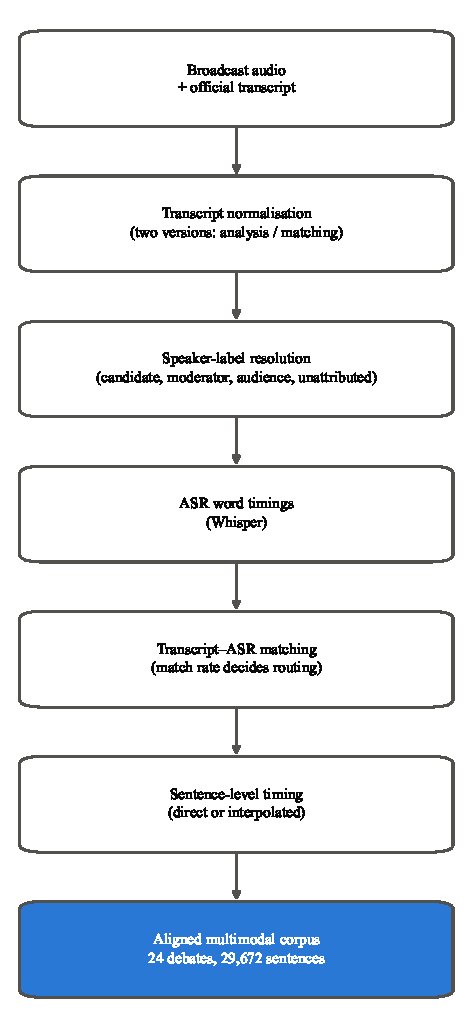
\includegraphics[width=0.72\columnwidth]{figures/fig_pipeline.pdf}
  \caption{Corpus construction pipeline. The match rate between the
  official transcript and recognised speech, computed before any analytical
  decision, determines whether a debate is routed to direct timing or
  interpolation (Table~\ref{tab:align}).}
  \label{fig:pipeline}
\end{figure}

Every acoustic measurement needs to know which piece of audio corresponds to
which sentence. This is the hardest practical step, because the transcripts
are not equally faithful. Some were produced verbatim, and others were tidied
for readability. Rather than assume, we measure. For each debate we run speech
recognition on the audio and count how many words of the official transcript
also appear, in order, in the recognised text. This match rate is computed
before any decision is taken. It determines how the debate is handled
(Table~\ref{tab:align}). Where the match is high, the official transcript is
treated as authoritative. Shared words take their timings directly, and the
gaps between them are filled by interpolation. Where it is lower, the same
method applies with more interpolated timing.

\begin{table}[t]
\caption{How the transcript was matched to the audio, decided by the measured
match rate before any analysis.}
\label{tab:align}
\centering
\begin{tabular}{lrrr}
\toprule
Treatment & Debates & Sentences & Match rate \\
\midrule
High fidelity     & 22 & 25{,}693 & $88.4$--$93.3\%$ \\
Reduced fidelity  & 2  & 3{,}979  & $69.7$--$82.3\%$ \\
\midrule
\textbf{Total}    & \textbf{24} & \textbf{29{,}672} & --- \\
\bottomrule
\end{tabular}
\end{table}

Forced alignment was also run and worked on $20$ of the $24$ debates. We still
used the recognition-based method throughout, for a design reason. If $20$
debates took timings from one method and four from another, the corpus would
carry a difference in timing accuracy that lines up with the age of the
recording, and therefore with the period. That is exactly the confound the
analysis is built to remove. One method everywhere avoids it. The forced alignment
output is kept as an independent check (Appendix~\ref{app:align}).

Each sentence then receives measurements at four levels: linguistic,
semantic, discourse and acoustic. These are detailed, tools and all, in
Section~\ref{sec:method:measures}.

\subsection{Quality Control and Exclusions}
\label{sec:data:quality}

Of the $24{,}193$ candidate sentences, $23{,}109$ ($95.5\%$; $10{,}868$
winning, $12{,}241$ non-winning) carry complete acoustic measurements. The
$1{,}084$ missing are $846$ sentences shorter than the $300$~ms extraction
floor plus $238$ extraction errors. Missing data is even across the two
outcome groups ($4.3\%$ against $4.7\%$), but it is very uneven across
alignment treatments ($2.8\%$ against $16.5\%$). This unevenness is one of
several reasons every statistical model below fits one term per debate
(Section~\ref{sec:method:fe}). Fitting one term per debate removes any
difference between debates, including this one, from the comparison of
interest. No two candidate sentences overlap in time, so
interruptions and overlapping speech are not represented anywhere in the
corpus. Appendix~\ref{app:known} lists the remaining known data-quality
issues (near-duplicate sentences, zero-duration rows, extraction failures) in
full.

\subsection{Final Corpus Statistics and Speaker Structure}
\label{sec:data:stats}

\begin{table}[t]
\caption{Who speaks in the corpus.}
\label{tab:roles}
\centering
\begin{tabular}{lrr}
\toprule
Speaker role           & Sentences & Share \\
\midrule
Candidate, winning     & 11{,}355 & $38.3\%$ \\
Candidate, non-winning & 12{,}838 & $43.3\%$ \\
Moderator              & 5{,}192  & $17.5\%$ \\
Audience               & 287      & $1.0\%$ \\
\midrule
\textbf{Total}         & \textbf{29{,}672} & $100\%$ \\
\bottomrule
\end{tabular}
\end{table}

\begin{table}[t]
\caption{Candidate sentences by election cycle.}
\label{tab:corpus}
\centering
\begin{tabular}{lrrr}
\toprule
Cycle & Debates & Winning & Non-winning \\
\midrule
1988 & 2 & 821    & 770    \\
1992 & 3 & 832    & 2{,}058 \\
1996 & 2 & 816    & 1{,}270 \\
2000 & 3 & 1{,}625 & 1{,}192 \\
2004 & 3 & 1{,}458 & 1{,}569 \\
2008 & 3 & 1{,}189 & 1{,}302 \\
2012 & 3 & 1{,}227 & 1{,}733 \\
2016 & 3 & 2{,}035 & 1{,}250 \\
2020 & 2 & 1{,}352 & 1{,}694 \\
\midrule
\textbf{Total} & \textbf{24} & \textbf{11{,}355} & \textbf{12{,}838} \\
\bottomrule
\end{tabular}
\end{table}

The corpus holds $29{,}672$ time-aligned sentences (Table~\ref{tab:roles}), of
which candidate sentences---the analytical population---are $81.5\%$.
Table~\ref{tab:corpus} gives the breakdown by election. The two groups differ
in size for two reasons: candidates get different amounts of floor time, and
in 1992 three people shared the stage, two of whom lost. This does not affect the
analysis, since every debate contributes both groups and all comparisons are
made within debates.

One statistic does not appear in either table. It governs the interpretation
of every result in this paper: these $24{,}193$ sentences come from
\textbf{$14$ people}. Twelve of them contested a single election, so they
appear in one outcome group only. This is not a minor limitation stated in
passing. Sections~\ref{sec:method:generalise} and~\ref{sec:disc:identity}
show in detail why it governs whether any predictive result can be trusted.
Table~\ref{tab:speakers} gives the structure.

\begin{table}[t]
\caption{Who is in the corpus. Twelve of fourteen candidates appear in only
one outcome group; two appear in both.}
\label{tab:speakers}
\centering
\footnotesize
\setlength{\tabcolsep}{4pt}
\begin{tabular}{lrrrr}
\toprule
Speaker & \multicolumn{2}{c}{Debates} & \multicolumn{2}{c}{Sentences} \\
\cmidrule(lr){2-3}\cmidrule(lr){4-5}
        & Win & Lose & Win & Lose \\
\midrule
Donald Trump        & 3 & 2 & 2{,}035 & 1{,}694 \\
George W.\ Bush     & 6 & 0 & 3{,}083 & --- \\
Barack Obama        & 6 & 0 & 2{,}416 & --- \\
George H.\,W.\ Bush & 2 & 3 & 821     & 1{,}034 \\
Bill Clinton        & 5 & 0 & 1{,}648 & --- \\
Mitt Romney         & 0 & 3 & ---     & 1{,}733 \\
John Kerry          & 0 & 3 & ---     & 1{,}569 \\
Joe Biden           & 2 & 0 & 1{,}352 & --- \\
John McCain         & 0 & 3 & ---     & 1{,}302 \\
Bob Dole            & 0 & 2 & ---     & 1{,}270 \\
Hillary Clinton     & 0 & 3 & ---     & 1{,}250 \\
Al Gore             & 0 & 3 & ---     & 1{,}192 \\
Ross Perot          & 0 & 3 & ---     & 1{,}024 \\
Michael Dukakis     & 0 & 2 & ---     & 770 \\
\midrule
\textbf{Total}      & \textbf{24} & \textbf{24} & \textbf{11{,}355} & \textbf{12{,}838} \\
\bottomrule
\end{tabular}
\end{table}

\subsection{Descriptive Profile of Candidate Speech}
\label{sec:data:descriptive}

Before applying the within-debate framework of Section~\ref{sec:method}, we
report a purely descriptive, pooled profile of candidate speech in the
Analytical Corpus: group means and percentages with no debate or speaker
controls. We include it because several of these pooled contrasts shrink or
reverse once the same comparisons are made within debates and checked
against speaker identity (Sections~\ref{sec:method:linguistic}--\ref{sec:method:acoustic}).
The gap between the pooled picture and the validated one is itself
informative: it shows how easily an uncontrolled comparison can mislead in
this corpus. This is why we report both profiles rather than only the
validated one.

Table~\ref{tab:descprofile} profiles sentence form, syntactic complexity and
lexical composition. Declarative sentences dominate both groups (about
$93\%$ of utterances). Winning candidates use somewhat more imperatives
($3.30\%$ against $2.62\%$) and slightly longer sentences ($14.03$ against
$13.60$ words). They also show more clausal material, marginally deeper
parses, slightly more nouns and adjectives, and slightly fewer third-person
pronouns. Lexical diversity and readability are essentially identical between
the two groups, and mean sentiment is mildly positive for both. Among the
$35$ Empath topic categories, winning candidates score higher on governance-
and policy-related themes (\emph{business}, \emph{economics}, \emph{money},
\emph{government}, \emph{law}, \emph{help}), and non-winning candidates
score higher on \emph{leader} and \emph{violence}. The absolute differences
are small throughout.

\begin{table}[t]
\caption{Descriptive profile of candidate speech in the Analytical Corpus:
pooled means or percentages per sentence, with no debate or speaker
controls.}
\label{tab:descprofile}
\centering
\footnotesize
\begin{tabular}{lrr}
\toprule
 & Winning & Non-winning \\
\midrule
Declarative sentences (\%)   & 92.86 & 93.57 \\
Imperative sentences (\%)    & 3.30  & 2.62  \\
\midrule
Words per sentence           & 14.03 & 13.60 \\
Clauses per sentence         & 1.84  & 1.74  \\
Subordinate/clausal material & 1.41  & 1.26  \\
Parse-tree depth             & 5.25  & 5.13  \\
\midrule
Type--token ratio            & 0.920 & 0.919 \\
Nouns (\% of tokens)         & 13.3  & 12.8  \\
Adjectives (\% of tokens)    & 4.9   & 4.5   \\
Third-person pronouns (\%)   & 3.9   & 4.2   \\
Flesch--Kincaid grade level  & 6.61  & 6.41  \\
Mean compound sentiment      & 0.086 & 0.070 \\
\bottomrule
\end{tabular}
\end{table}

In the discourse layer, statements dominate as expected ($93.2\%$ of
candidate sentences carry the statement tag; informational statements
$9.6\%$, explanations $6.2\%$, personal stance $5.5\%$, patriotic appeals
$4.8\%$). Table~\ref{tab:tagdiff} lists the categories with the largest
pooled win/non-win frequency differences. Winning candidates use more
interactive and explanatory acts (imperatives, explanations, agreement,
rejection, direct answers). Non-winning candidates use more
rhetorical framing (patriotic appeals, historical references, emotional
appeals, unity framing). Section~\ref{sec:method:discourse} shows that
several of these categories are dominated by single lexical triggers, so we
read this table as descriptive of the annotation layer rather than as a
validated behavioural difference.

\begin{table}[t]
\caption{Discourse-act and rhetorical categories with the largest absolute
pooled frequency differences between outcome groups (percentage of
candidate sentences; uncontrolled for debate or speaker).}
\label{tab:tagdiff}
\centering
\footnotesize
\setlength{\tabcolsep}{3pt}
\begin{tabular}{llrrr}
\toprule
Category & Type & Winning & Non-win.\ & $\Delta$ \\
\midrule
Patriotic appeal     & Rhetorical   & 4.29 & 5.18 & $-0.89$ \\
Imperative/directive & Dialogue act & 3.30 & 2.62 & $+0.68$ \\
Explanation          & Dialogue act & 6.44 & 5.91 & $+0.53$ \\
Agreement            & Dialogue act & 1.16 & 0.77 & $+0.40$ \\
Historical reference & Rhetorical   & 0.84 & 1.21 & $-0.36$ \\
Emotional appeal     & Rhetorical   & 1.51 & 1.81 & $-0.30$ \\
Rejection            & Dialogue act & 0.85 & 0.62 & $+0.23$ \\
Yes--no question     & Dialogue act & 0.55 & 0.74 & $-0.20$ \\
Direct answer        & Dialogue act & 1.11 & 0.93 & $+0.18$ \\
Unity framing        & Rhetorical   & 1.50 & 1.64 & $-0.14$ \\
\bottomrule
\end{tabular}
\end{table}

Acoustically, the same pooled comparison shows winning candidates pausing
more (mean total pause time $0.402$~s against $0.290$~s per sentence;
$1.02$ against $0.77$ pauses) at a slightly higher syllable rate ($5.64$
against $5.51$ syllables/s). Section~\ref{sec:method:acoustic} shows that
this pausing difference does not survive removing a single speaker: exactly
the kind of gap between the pooled and validated pictures noted above.

%=======================================================================
\section{Analytical and Experimental Framework}
\label{sec:method}
%=======================================================================

\subsection{Outcome and Unit of Analysis}
\label{sec:method:unit}

Every candidate--debate record carries a binary outcome label, defined as
follows:
\begin{equation}
w_{d,s} =
\begin{cases}
1, & \text{ticket } s\text{ won the election after debate } d, \\
0, & \text{otherwise.}
\end{cases}
\label{eq:outcome}
\end{equation}
We use three units of analysis. \emph{Sentence level} is the finest grain,
used for the statistical screen (Section~\ref{sec:method:fe}) and for
training classifiers (Section~\ref{sec:method:forest}). Measurements exist at
this level, but the outcome label does not. The label is assigned once per
candidate--debate, so all sentences from one candidate in one debate share
one label. \emph{Candidate-by-debate} is the aggregate used wherever speaker
identity itself is the variable of interest (Table~\ref{tab:speakers};
Section~\ref{sec:method:generalise}). \emph{Debate-level paired prediction}
asks, for a whole debate, whether the model's aggregate score ranks the
winning candidate above the opponent. Every generalisation claim in
Sections~\ref{sec:method:generalise} and~\ref{sec:method:llm} is judged at
this level, because it is the only one of the three not affected by class
imbalance or by dependence between sentences from the same speaker.

\subsection{Broad Multimodal Measure Set}
\label{sec:method:measures}

We measure each sentence at four levels: linguistic, semantic, discourse
and acoustic. Together these come to $43$ measures; the complete dictionary
is in Appendix~\ref{app:features}. The next four subsections describe how
each level is built, in the order a sentence passes through the pipeline:
what it says, what it means, what it does as an utterance, and how it
sounds.

\subsubsection{Linguistic Representation}
\label{sec:method:linguistic-rep}

Sentence-level parsing and part-of-speech tagging use spaCy
(\texttt{en\_core\_web\_sm}) \cite{honnibal2020spacy}. We classify sentence
form (declarative, interrogative, imperative, exclamatory) from punctuation
and dependency rules. We measure structural complexity with clause count,
parse-tree depth, and mean dependency length. Clause-related counts come
from the dependency relations \texttt{ccomp}, \texttt{xcomp},
\texttt{advcl}, \texttt{acl} and \texttt{relcl}. This set includes some
non-finite complements, so we read the resulting count as \emph{clausal
material} rather than as a literal subordinate-clause count;
Section~\ref{sec:method:linguistic} shows why that distinction matters once
the numbers come in. Lexical measures are sentence length, mean word
length, type--token ratio, the balance of function to content words,
part-of-speech proportions, and separate first-, second- and third-person
pronoun rates. Readability is four scores: Flesch Reading Ease,
Flesch--Kincaid Grade Level, SMOG, and Gunning Fog.

\subsubsection{Semantic Representation}
\label{sec:method:semantic-rep}

We estimate sentence-level sentiment with VADER: compound polarity, plus
separate positive, negative and neutral components \cite{hutto2014vader}.
We measure topic content with $35$ Empath categories \cite{fast2016empath},
chosen before we ran any outcome analysis, to represent politically
relevant themes. We treat these as a semantic diagnostic family, not as
$35$ additional primary hypotheses. We represent contextual meaning with
$384$-dimensional Sentence-BERT embeddings (\texttt{all-MiniLM-L6-v2})
\cite{reimers2019sbert}, used only for exploratory analysis, since no
single dimension of an embedding has a direct linguistic interpretation.

\subsubsection{Discourse Annotation: DAMSL and BEADS}
\label{sec:method:discourse-rep}

Dialogue acts follow the DAMSL framework \cite{core1997damsl}. We
complement it with BEADS, a framework of rhetorical and bias-related
categories we built for political debate speech: personal stance,
patriotic appeal, fear appeal, historical reference, unity framing, and
others \cite{prahallad2025beads}. The combined scheme has $28$ dialogue-act
categories and $21$ BEADS categories, and it is multi-label: one sentence
can carry more than one tag. The full tag inventory, with definitions and
worked examples, is documented separately \cite{prahallad2025beads}. We
generate primary annotations with a transparent, rule-based tagger that
combines sentence form, lexical and phrase patterns, question structure
(auxiliary inversion for yes--no questions, interrogative words for
wh-questions), and first-person stance markers. We also generate an
independent, model-based annotation as a second measurement instrument.
Section~\ref{sec:method:discourse} treats agreement between the two as a
measurement-validity question, and treats neither one as
human-adjudicated ground truth.

\subsubsection{Acoustic Representation}
\label{sec:method:acoustic-rep}

Acoustic measures are average pitch, its variation, range and slope,
computed both in hertz and on a semitone scale. A hertz-based measure of
variation grows with average pitch automatically, so the semitone scale is
needed for a fair comparison across speakers. Acoustic measures also
include loudness and its variation; three measures of the voice source,
including harmonic-to-noise ratio computed by two independent tools;
silent-pause count, total duration and average duration; and speech and
articulation rate in words and syllables. Appendix~\ref{app:tools} lists
every tool, version and parameter setting behind these four subsections.

\subsection{Targeted Pitch-Contour Measure Set}
\label{sec:method:pitch:extract}

Section~\ref{sec:method:acoustic} shows that narrower semitone pitch range is
the one acoustic property that survives every validity check in the broad
screen. Every measure up to that point treats pitch variability as a single
number per sentence---a standard deviation, or the width of a percentile
band. Such a number answers \emph{how much} a speaker's pitch moves and says
nothing about the \emph{shape} of that movement. We therefore extract the
pitch contour itself and build ten further measures of its shape and
dynamics, as a targeted follow-up on the one construct already established
by the broad screen.

For each candidate sentence we recover the frame-level semitone-scaled pitch
contour. This is the same quantity summarised by the surviving broad-screen
measure, but recovered before it is collapsed to one number. We extract it
using the openSMILE eGeMAPSv02 low-level descriptor
\texttt{F0semitoneFrom27.5Hz\_sma3nz} at its native $10$~ms frame rate,
extracted independently per sentence clip to match the original per-clip
procedure exactly. We validate this extraction against the already published
semitone functionals for $1{,}000+$ sentences and find the two agree to
within floating-point rounding (mean absolute difference $0.0006$). A
sentence needs at least $10$ voiced frames ($100$~ms of voiced speech) to be
included. This is a floor rather than a guarantee of reliability, so we
additionally assess reliability by stratifying on duration after the fact,
the same way we do for voice clarity in Section~\ref{sec:method:acoustic}.

From the voiced frames of each sentence we compute ten measures in two
groups. \emph{Distributional shape} measures are order-independent.
\emph{Skewness} indicates whether the distribution leans toward higher or
lower pitch, with a longer tail on one side. \emph{Kurtosis} indicates
whether frames cluster near a central value with occasional large
excursions, or instead spread more evenly across the range. The
\emph{interquartile-to-range ratio} is the width of the middle half of the
distribution relative to its $20$--$80$ percentile span. \emph{Dynamics}
measures are order-dependent: they are computed only across pairs of
consecutive voiced frames, so no estimate spans a silent or unvoiced gap.
\emph{Pitch velocity} is the mean and standard deviation of the
frame-to-frame semitone change. \emph{Pitch acceleration} is the mean
absolute second difference. \emph{Turning points per second} is how often
the contour changes direction. \emph{Total variation} is the summed absolute
frame-to-frame movement normalised by voiced duration. Finally, we fit a
linear trend to each sentence's contour and remove it; from this we compute
the \emph{declination slope} of that trend and the
\emph{declination-residual standard deviation}, which is the spread of
whatever pitch movement is left once the sentence's overall rise or fall is
subtracted out. We evaluate all ten with the statistical design of
Section~\ref{sec:method:fe}, applying Benjamini--Hochberg correction at
$q = 0.05$ across this family of ten measures. This family is kept separate
from the broad-screen family of $43$.

\subsection{Within-Debate Statistical Comparison}
\label{sec:method:fe}

Every analysis in this paper, broad screen and targeted follow-up alike,
uses one statistical design, described once here.

\emph{Comparing within debates.} For each measure $y$ and sentence $i$, with
$w_i = 1$ for winning candidates, we fit
\begin{equation}
y_i \;=\; \beta w_i \;+\; \sum_{d} \alpha_d D_{i,d} \;+\; \varepsilon_i \,,
\label{eq:fe}
\end{equation}
where $D_{i,d}$ marks sentence $i$ as belonging to debate $d$. One term per
debate removes everything that varies between debates, so $\beta$ is the
difference \emph{inside} debates. It is free of differences in period,
format, equipment, moderator, and topic. We report $\beta/\sigma_{\text{within}}$, the
difference in standard deviations.

\emph{Uncertainty and $p$-values.} We compute cluster-robust standard
errors, treating each debate as a cluster and, separately, treating each
speaker as one. Every effect carries a $95\%$ confidence interval. Our
primary $p$-value is an exact randomization test: we flip the winner label
within each debate and recompute the effect. With $24$ debates there are
$2^{24} = 16{,}777{,}216$ possible flips, and we enumerate all of them.

\emph{Correcting for multiple measures.} With $43$ measures, about two would
clear $p < 0.05$ by chance alone. We control the false discovery rate at
$q = 0.05$ with the Benjamini--Hochberg procedure
\cite{benjamini1995controlling}: we sort the $p$-values smallest first and
compare the $k$-th against $k \times 0.05/43$.

\emph{Asking whether a result would repeat.} We pool the $24$ debates with a
random-effects model. We report how much the effect varies between debates
($I^2$), a $95\%$ confidence interval for the average, and a $95\%$
\emph{prediction interval} for a new debate. $I^2$ is the percentage of the
total variation across debates that reflects real differences between
debates rather than sampling noise; $0\%$ means the debates agree up to
noise, and values near $100\%$, which is what we find throughout this
paper, mean the effect size itself swings from debate to debate. The
confidence interval answers what the average difference was across the
debates we have. The prediction interval answers whether we would see the
difference at all in a debate we have not.

\subsection{Measurement-Validity Protocol}
\label{sec:method:validity}

Significance and multiple-comparison correction are not sufficient grounds to
call a measure reliable. We therefore require every candidate measure in this
paper to clear seven further checks before it is reported as reliable rather
than merely detected:

\begin{enumerate}\itemsep2pt
  \item \textbf{Speaker coupling.} Does the measure correlate with a
        speaker's own habitual pitch, across speakers and within a single
        speaker's own debates (Sections~\ref{sec:method:acoustic},
        \ref{sec:method:pitch})?
  \item \textbf{Cross-implementation agreement.} Does it agree across
        independent tools measuring the same quantity (Praat versus
        openSMILE; Section~\ref{sec:method:acoustic})?
  \item \textbf{Duration reliability.} Is it reliable across the range of
        sentence durations actually present in the corpus
        (Table~\ref{tab:reliab})?
  \item \textbf{Alignment-treatment stability.} Does it hold sign under both
        the high- and reduced-fidelity alignment treatments
        (Table~\ref{tab:align})?
  \item \textbf{Leave-one-speaker-out stability.} Does it retain direction
        when each speaker in turn is removed and the effect recomputed?
  \item \textbf{Cross-debate recurrence.} Does it appear in a majority of the
        $24$ debates individually, not only in the pooled average?
  \item \textbf{Prediction-interval support.} Does its $95\%$ prediction
        interval for a new debate exclude zero?
\end{enumerate}
Section~\ref{sec:method:acoustic} reports the largest observed effect in the
paper failing checks 1--2. Section~\ref{sec:method:pitch} reports the primary
finding passing checks 1--6 and failing check 7. We treat this as the
paper's central qualification rather than a caveat appended to it.

\subsection{Generalisation Protocol}
\label{sec:method:genprotocol}

We use two evaluations throughout, and they answer different questions.
\textbf{Debate held out}: the debate under test is absent from training, but
its speakers' other debates may remain. This is the standard setup in most
published work. \textbf{Speakers held out}: every debate containing either
of the test debate's speakers is absent from training, so neither
candidate's voice appears anywhere in the model. We treat the second as the
primary evaluation of generalisation in this paper. We also report the first
alongside it, because the gap between the two is itself the result we report
in Section~\ref{sec:method:generalise}.

\subsection{LLM Evaluation Protocol}
\label{sec:method:llmprotocol}

For each of the $24$ debates we build an anonymised record. Every candidate
sentence has its names, party, and the date removed. Each candidate is
relabelled \emph{Candidate A}, \emph{B}, or \emph{C}, in an order that is
re-randomised on every repeat. We ask the model (Anthropic's
\texttt{claude-opus-4-8}; full specification in Appendix~\ref{app:llmrepro})
which candidate went on to win that year's election. We ask this under two
conditions, both built from the same $34$ of the $43$ measures used in
Section~\ref{sec:method:combined} (those with complete values on enough
rows). In the \textbf{transcript} condition the model sees only the
anonymised candidate turns, in order, and nothing else. In the
\textbf{descriptors} condition it sees the $34$ within-debate standardised
measures, averaged per candidate, as a table, with no transcript text at
all. We also run a third condition with both together. It agrees with the
transcript-only condition on all $24$ debates, so we report it only in
Appendix~\ref{app:supplement}.

Every call also requires a short explanation and up to five cited reasons.
Each reason is drawn from a closed vocabulary: the $34$ measure names for
the descriptor condition, or eight qualitative themes for the transcript
condition. This closed vocabulary means a citation can be checked by machine
against the real data, rather than read and judged by hand. We run two further checks
alongside the prediction itself. A \textbf{contamination probe} sends the
model the same anonymised input, with no prediction question at all, and
asks it to identify the specific debate. A \textbf{grounding check} compares
every cited measure against the real standardised value for that debate. We
score each debate three times per condition, re-randomising the candidate
letters each time.

%=======================================================================
\section{Broad Multimodal Screening}
\label{sec:method:screen}
%=======================================================================

This section answers RQ1: which properties differ, within debates, between
winning and non-winning candidates, across $43$ measures at four levels. It
is also where the pooled, uncontrolled comparison of
Section~\ref{sec:data:descriptive} meets the validated one. Several of the
contrasts in Tables~\ref{tab:descprofile} and~\ref{tab:tagdiff} shrink,
disappear or reverse once the same measures are compared within debates. We
flag each case as it comes up below. Figure~\ref{fig:effects}, at the end of
this section, plots all $43$ measures side by side; the prose below walks
through what is in it, level by level, and Table~\ref{tab:acousticsummary}
gives a one-line verdict on each of the three acoustic patterns that stand
out in it.

\subsection{Linguistic and Semantic Results}
\label{sec:method:linguistic}

Before reading any result from the subordination counter, one property of it
must be stated. It accepts dependency relations that admit non-finite
complements, and it reports $1.41$ subordinate clauses out of $1.84$ total
in a fourteen-word sentence. This is too high to be real subordination, so
we read this measure as ``clausal material'' rather than subordination.

\emph{Sentence structure.} The pattern here is weak and points one way.
Table~\ref{tab:sentstruct} gives the four measures side by side: winning
candidates produce slightly more clausal material on every one of them, but
none of these effects survives correction, and every confidence interval
includes zero. The effects are also two to eight times larger in the
reduced-fidelity treatment, which places most of them in two debates from
one cycle rather than across the corpus.

\begin{table}[t]
\caption{Sentence-structure measures: within-debate effect size, in
standard deviations. Positive means higher among winning candidates. None
survives Benjamini--Hochberg correction.}
\label{tab:sentstruct}
\centering
\begin{tabular}{lr}
\toprule
Measure & Effect \\
\midrule
Subordinate clauses (clausal material) & $+0.093$ \\
Clause count                           & $+0.086$ \\
Sentence length                        & $+0.034$ \\
Parse depth                            & $+0.029$ \\
\bottomrule
\end{tabular}
\end{table}

\emph{Words and semantics.} Adjective rate is the strongest single text
measure, at $+0.062$ ($p = 0.0036$). It misses correction by a hair. It
clears correction in any family of $41$ measures or fewer, but not in $43$.
We report it without explanation, since we had no prior expectation about
adjectives. This is the one measure in this section where the pooled and
the validated comparison agree in direction. Table~\ref{tab:descprofile}
already showed winning candidates using more adjectives ($4.9\%$ against
$4.5\%$ of tokens), with no debate or speaker controls at all. The
within-debate effect points the same way, even though it does not survive
correction. Pronouns do not separate the groups at all: second person
$-0.048$, third person $+0.009$, first person $-0.003$. Third
person is the case where pooled and validated comparison disagree. The raw
pooled numbers of Table~\ref{tab:descprofile} put winning candidates
\emph{lower} ($3.9\%$ against $4.2\%$). This is the opposite sign from the
within-debate effect above, which is itself indistinguishable from zero.
Neither number
supports a real difference, but the sign flip between them is a useful
warning: a pooled comparison this small can point either way depending on
which debates happen to carry more of each group. We record the pronoun
null on its own, because in a debate \emph{you} nearly always means the
opponent: if these two groups differ, it is not in how much they address
each other. Readability and sentiment do not separate the groups either
($+0.030$, $p = 0.27$).

\emph{The embedding axis.} We draw the line between the two groups' average
sentence vectors and sort the corpus along it. This produces a striking
result: the $50$ highest-scoring sentences split $40$ to $10$ between
winning and non-winning candidates, a stronger separation than anything else
in this section. A closer look at these sentences shows that this split does not, in fact,
reflect a separation between the groups. Among the $200$ highest-scoring sentences,
$47.5\%$ contain \emph{she}, \emph{her} or \emph{hers}, against $1.9\%$ in
the corpus overall. Of the top $50$ sentences, $32$ come from one candidate
and $29$ from the 2016 cycle. The axis separates talking about a female
opponent from talking about past presidents, in one election. It is not a
sentence-length axis either: the correlation is $+0.09$, and removing
length leaves the poles unchanged. We report this as a diagnostic of what a single
difference-of-centroids direction can produce by accident, not as a finding:
following Biber \cite{biber1988variation}, a register dimension would have
to be recovered from many co-occurring features across texts.

\subsection{Discourse-Measure Validity}
\label{sec:method:discourse}

This layer produced no usable result. The reason lies in the instrument,
not in the underlying construct. Table~\ref{tab:tagdiff} already
showed pooled, uncontrolled frequency differences of up to $0.89$
percentage points on exactly these categories, with patriotic appeal,
historical reference and unity framing all higher among non-winning
candidates. The following audit is why we do not read that table as a
behavioural finding. We check what fraction of each category's hits come
from a single string. Several of the rule-based detectors turn out to be
keyword matchers rather than concept detectors. Unity framing and patriotic
appeal are dominated by the strings \emph{United States} and
\emph{America}/\emph{American}. Historical reference is dominated by a bare
four-digit year. Fear appeal is dominated by unbounded substring matches.
Table~\ref{tab:ruleaudit} audits the four fixable categories directly.
Fixing the rules removes $94$--$97\%$ of what these categories had counted.
What survives appears in under $0.5\%$ of sentences, with differences no
larger than $0.014$.

\begin{table}[t]
\caption{Audit of four rule-based discourse detectors. ``Sole trigger'' is
the share of hits produced by the listed string alone. ``Repaired'' is the
count after anchoring the rule to that string at a word boundary, with the
effect recomputed on what survives.}
\label{tab:ruleaudit}
\centering
\footnotesize
\setlength{\tabcolsep}{3pt}
\begin{tabular}{lrlrr}
\toprule
Category & Orig.\ & Dominant trigger & Sole & Repaired \\
         & hits   &                  & trigger & (hits, effect) \\
\midrule
Unity framing    & 396   & ``United States''  & $80.1\%$ & 69, $-0.004$ \\
Patriotic appeal & 1{,}235 & ``America''      & $88.0\%$ & 115, $-0.014$ \\
Historical ref.\ & 265   & four-digit year    & $63.4\%$ & 165, $-0.028$ \\
Fear appeal      & 540   & substring match    & $30.9\%$ & 373, $+0.007$ \\
\bottomrule
\end{tabular}
\end{table}

A second, independent labelling by a large language model agrees with the
rule-based one at chance on the interpretive, rhetorical categories
(Krippendorff's $\alpha = +0.012$), and only modestly better on the more
grammatically observable dialogue acts ($\alpha = +0.199$). A
chain-of-thought variant of the same prompt does not close this gap. We
draw no conclusion about rhetorical strategy from this layer anywhere in
this paper. The full trigger audit, category-level agreement table, and
chain-of-thought comparison are in Appendix~\ref{app:tagging}
(Table~\ref{tab:regex}).

\subsection{Acoustic Results}
\label{sec:method:acoustic}

Following K\"unzel \cite{kunzel1989speakers}, we treat average pitch as weak
evidence when comparing different people. We treat variation as more
meaningful, since variation describes what a speaker does rather than what
their larynx is. Any measure that correlates with a speaker's own average
pitch is therefore suspect, and we test each one for this correlation.

\emph{The two measures that survive.} The semitone pitch range between the
$20$th and $80$th percentiles averages $4.51$ for winning candidates and
$4.91$ for non-winning ones: winners move their pitch across a narrower
band. The difference is $-0.226$ standard deviations, confidence interval
$(-0.332, -0.120)$, randomization $p = 0.00017$, present in $21$ of $24$
debates. Dropping any one speaker leaves it between $-0.308$ and
$-0.169$, always the same sign. It holds in both alignment treatments
($-0.229$ and $-0.206$). It barely correlates with a speaker's own average
pitch ($r = +0.11$). Correcting for average pitch makes it
\emph{stronger} ($-0.267$). The second measure, pitch variation relative to
average pitch, is larger ($-0.332$, $p = 8.8\times10^{-6}$, $20/24$) but
less clean. It correlates with a speaker's average pitch at $r = -0.49$,
and it collapses to $+0.021$ in the reduced-fidelity treatment. We treat the
percentile range as primary and the ratio as corroborating, a choice made on
measurement quality rather than on $p$-values. Both measures survive
Benjamini--Hochberg correction and would survive the stricter Bonferroni
threshold.

\emph{Voice clarity: the largest effect, and what it measures.} The biggest
single effect in the study is harmonic-to-noise ratio: $+0.461$ on one tool,
$+0.315$ on the other. At face value, winners have clearer voices. The
validity checks say we cannot tell what it measures. Across the fourteen
speakers, average pitch correlates with average harmonic-to-noise ratio at
$r = +0.776$ on one tool and $+0.896$ on the other. Ranking the speakers by
voice clarity nearly reproduces the ranking by pitch, most likely because a
fixed $60$~ms analysis window gives a low-pitched voice fewer cycles to work
with, and because television transmission cuts low frequencies. The two
tools then behave differently under a within-speaker check. In $51$
speaker-by-debate cells, the correlation collapses to a median of $+0.083$
for one tool. For the other tool, it stays at $+0.566$ and is positive in
all $51$ cells. Two standard tools for the same quantity should not disagree this
way if both are measuring voice quality. We take this as the clearest single
illustration in the paper of Section~\ref{sec:method:validity}'s checks
1--2: same family, same corpus, same statistics as the surviving
pitch-range measure, and this one fails both.

\emph{Pausing.} Winners pause more on every version of the measure ($+0.14$
to $+0.20$ across five variants), consistent across alignment treatments and
duration bins. The speaker check rules this out. \textbf{All six pause
measures change sign when Barack Obama is removed}, from $+0.196$ to
$-0.021$ for pause proportion. His three 2012 debates alone carry effects of
$+0.96$ to $+1.25$. The measure itself is sound. The finding is a
description of one person, not of winning candidates in general.

Table~\ref{tab:acousticsummary} puts the three patterns side by side. Only
the semitone percentile range clears every check; the other two look just
as strong, or stronger, on the numbers alone.

\begin{table}[t]
\caption{The three acoustic patterns of this section, and why only one
survives every check in Section~\ref{sec:method:validity}.}
\label{tab:acousticsummary}
\centering
\footnotesize
\setlength{\tabcolsep}{3pt}
\begin{tabular}{lrlp{0.28\textwidth}}
\toprule
Pattern & Effect & Debates & Verdict \\
\midrule
Semitone $20$--$80$ range & $-0.226$ & $21/24$ & Survives every check; the paper's primary broad-screen result \\
Semitone SD/mean & $-0.332$ & $20/24$ & Corroborating only; coupled to the speaker's own habitual pitch \\
Voice clarity (both tools) & $+0.461$ / $+0.315$ & $13/24$ & Fails; tracks the speaker's larynx, not behaviour \\
Pausing & $+0.14$ to $+0.20$ & $14/24$ & Fails; reverses when one speaker (Obama) is dropped \\
\bottomrule
\end{tabular}
\end{table}

Figure~\ref{fig:effects} shows all $43$ measures together.

\begin{figure*}[!t]
  \centering
  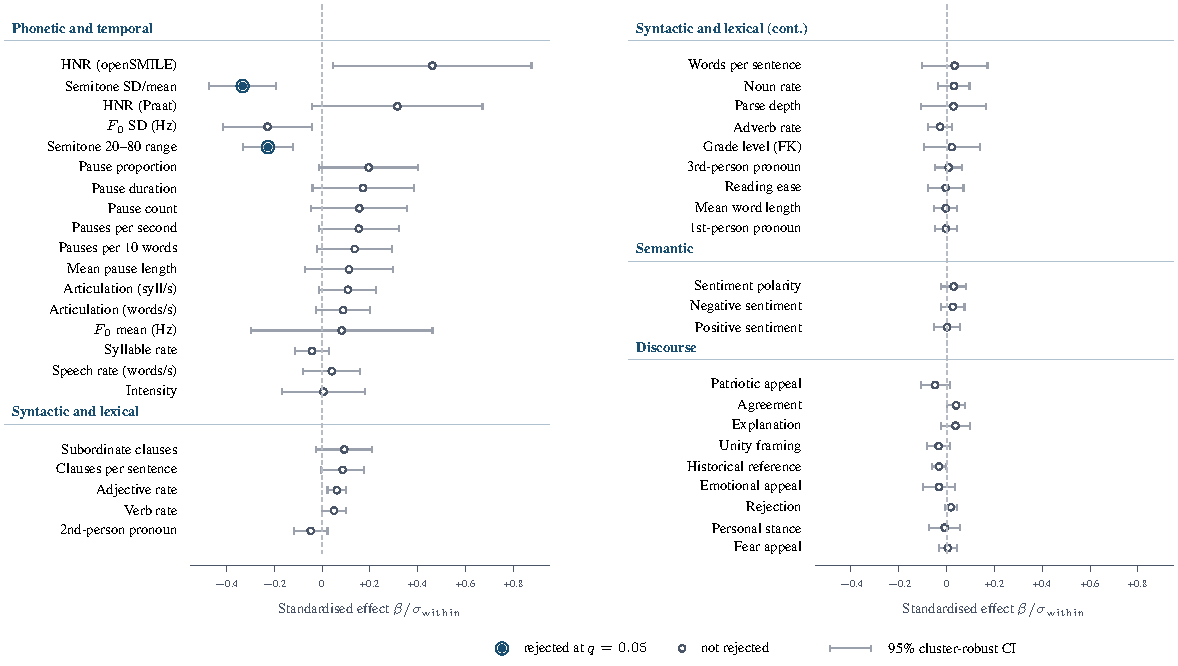
\includegraphics[width=0.99\textwidth]{figures/fig3_effects_v2.pdf}
  \caption{Within-debate difference for all $43$ measures, in standard
  deviations, with $95\%$ confidence intervals that account for clustering by
  debate. Positive means higher among winning candidates. Filled markers are
  the two measures that survive correction for multiple comparisons. Note the
  scale: the biggest effect is $0.46$ and most are under $0.05$.}
  \label{fig:effects}
\end{figure*}

%=======================================================================
\section{Residual Pitch Control: The Primary Finding}
\label{sec:method:pitch}
%=======================================================================

This section answers RQ2: what specific property of the pitch contour
accounts for the strongest and most robust acoustic difference.

\subsection{From Narrower Pitch Range to Residual Movement}
\label{sec:pitch:progression}

We build the result in four steps. First, the broad screen
(Section~\ref{sec:method:acoustic}) shows winning candidates use a narrower
semitone pitch band. Second, that number alone does not say what kind of
movement produces the narrower band: a flatter overall melody and a steadier
local wobble on top of the same melody would both shrink it. Third, the
frame-level measure set of Section~\ref{sec:method:pitch:extract} asks the
question directly, by removing each sentence's own linear rise or fall and
measuring what is left. Fourth, what is left is smaller for winning
candidates: a specifically \emph{local}, moment-to-moment difference in
pitch control, not a difference in overall prosodic sweep.
Figure~\ref{fig:schematic} illustrates the distinction with two synthetic
contours that share one sentence-level sweep and differ only in residual
movement.

\begin{figure}[t]
  \centering
  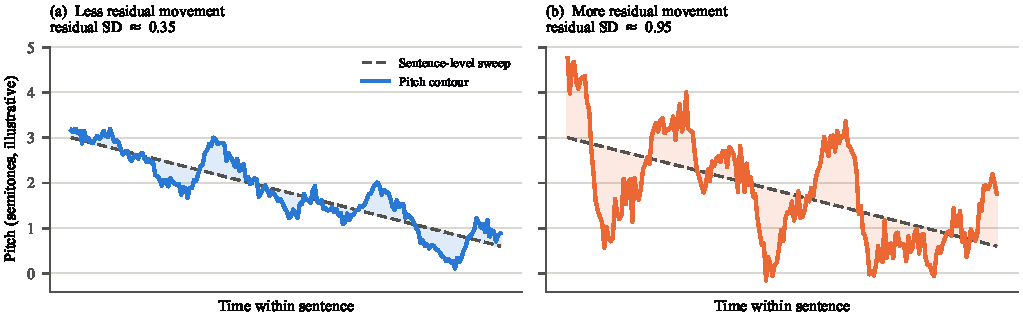
\includegraphics[width=\columnwidth]{figures/fig_schematic.pdf}
  \caption{What ``residual pitch movement'' means. Both panels share the same
  sentence-level sweep (dashed). The shaded area is the residual left over
  once that sweep is subtracted out. Synthetic illustration, not real corpus
  data.}
  \label{fig:schematic}
\end{figure}

\subsection{Primary Result}
\label{sec:pitch:primary}

\begin{figure}[t]
  \centering
  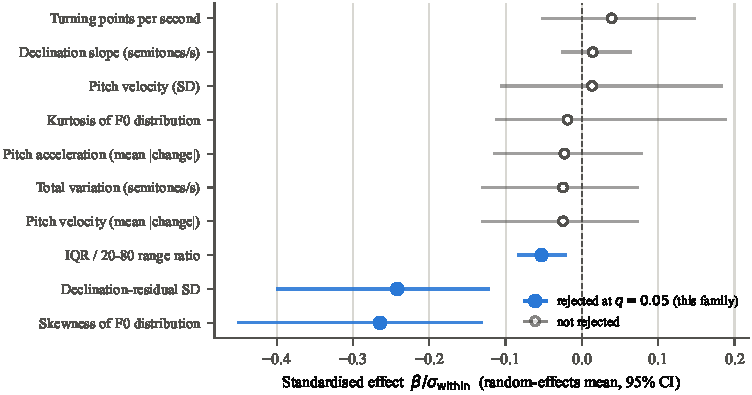
\includegraphics[width=\columnwidth]{figures/fig_tier12.pdf}
  \caption{Within-debate standardised effect (random-effects mean, $95\%$
  confidence interval) for the ten higher-order and dynamic pitch measures.
  Filled markers survive Benjamini--Hochberg correction within this family.}
  \label{fig:tier12}
\end{figure}

\begin{table}[t]
\caption{The ten pitch-contour measures. Effect is $\beta/\sigma_{\text{within}}$.
Dir.\ is debates in the pooled direction of $24$. $I^2$ is in per cent.
LOSO stable means the effect keeps its sign when each of the fourteen
speakers is dropped in turn (leave-one-speaker-out). PI is the $95\%$
prediction interval. Ordered by exact randomization $p$.}
\label{tab:tier12}
\centering
\scriptsize
\setlength{\tabcolsep}{2pt}
\begin{tabular}{lrrrrrr}
\toprule
Measure & Eff. & $p_{\text{perm}}$ & Dir. & $I^2$ & LOSO stable & BH \\
\midrule
Declination-residual SD  & $-0.242$ & $0.0005$ & $20/24$ & $96$ & yes & \tick \\
Skewness                 & $-0.265$ & $0.0014$ & $19/24$ & $97$ & yes & \tick \\
IQR / $20$--$80$ ratio   & $-0.053$ & $0.0036$ & $16/24$ & $24$ & yes & \tick \\
Turning points / sec     & $+0.039$ & $0.431$  & $12/24$ & $93$ & no  & \notick \\
Declination slope        & $+0.014$ & $0.492$  & $14/24$ & $65$ & no  & \notick \\
Pitch acceleration       & $-0.023$ & $0.667$  & $14/24$ & $92$ & no  & \notick \\
Pitch velocity (mean)    & $-0.025$ & $0.668$  & $13/24$ & $93$ & no  & \notick \\
Total variation          & $-0.025$ & $0.668$  & $13/24$ & $93$ & no  & \notick \\
Kurtosis                 & $-0.019$ & $0.796$  & $14/24$ & $97$ & no  & \notick \\
Pitch velocity (SD)      & $+0.013$ & $0.881$  & $14/24$ & $97$ & no  & \notick \\
\bottomrule
\end{tabular}
\end{table}

Table~\ref{tab:tier12} and Figure~\ref{fig:tier12} show that three measures
clear correction and seven do not. \textbf{Declination-residual standard
deviation is the cleanest result in the paper.} Winning candidates have less
pitch movement left over once each sentence's own linear rise or fall is
removed: effect $-0.242$, exact randomization $p = 0.0005$, present in $20$
of $24$ debates (sign-test $p = 0.0015$), sign-stable across all fourteen
leave-one-speaker-out refits. It passes the two checks that separated the
broad screen's two surviving measures from each other
(Section~\ref{sec:method:acoustic}). Correlation with a speaker's own mean
pitch is $r = -0.06$ across speakers and $r = +0.23$ within
speaker-by-debate cells. It is uncoupled by either reckoning, unlike the
confounded voice-clarity measure. Rather than shrinking with sentence length, the way a
noise artefact would, it \emph{grows}: from $-0.17$ in sentences under a
second to $-0.53$ in sentences over six. It holds sign in both alignment
treatments, more weakly in the reduced-fidelity group ($-0.26$ against
$-0.08$) but without reversing.

\subsection{Secondary Pitch-Shape Findings}
\label{sec:pitch:secondary}

\emph{Skewness} survives the same correction, but it fails the same check
that demoted the broad screen's secondary pitch measure. It correlates with
a speaker's own mean pitch at $r = -0.29$ across speakers and $r = -0.24$
within cells. It also reverses sign under alignment treatment ($-0.31$
against $+0.08$). By the same standard applied throughout, we report it as
corroborating rather than clean. \emph{The interquartile-to-range ratio} has
the lowest heterogeneity of any measure in this paper ($I^2 = 24\%$ against
$94$--$97\%$ elsewhere). It is stable across duration bins and alignment
treatment. Its per-debate sign count, however, is the weakest of the three
($16/24$, sign-test $p = 0.15$). It also shows the same across-speaker pitch
coupling as skewness ($r = -0.26$). We report it as secondary: consistent in
magnitude whenever it appears, but appearing less consistently than either
of the other two.

\subsection{What the Null Results Rule Out}
\label{sec:pitch:nulls}

Pitch velocity, acceleration, total variation and turning-point rate---every
measure of how quickly or how erratically the contour moves---show no
difference between the groups, with $I^2$ above $90\%$ throughout and
prediction intervals spanning zero by a wide margin. Kurtosis and the
declination slope itself show none either. Taken with the positive result
above, this rules out an entire class of explanation: it is not that
winning candidates move their pitch faster, more smoothly, or less
erratically. It is specifically that the \emph{spread} of where their pitch
sits is smaller. More precisely, it is the spread that remains after
removing each sentence's own trend that is smaller. The data therefore support a
distributional account of the effect rather than a kinematic one.

%=======================================================================
\section{Generalization, Speaker Confounding, and Contamination}
\label{sec:method:generalise}
%=======================================================================

This section answers RQ3 and RQ4 together, because they turn out to be the
same finding reached twice. Three classical models built on the measures of
Section~\ref{sec:method:screen} look like they predict the winner. A large
language model given the raw transcript looks like it does too. But all four
are actually detecting who is speaking, or which debate this is, not how
winners communicate. We treat this as a central result rather than a
limitation appended to one.

\subsection{Interpretable and Nonlinear Models}
\label{sec:method:combined}

If text and audio carry different information, combining them should carry
more than any single measure. We use two models that make different
assumptions about how measures combine: a linear discriminant, which uses
the full covariance structure, and a decision forest, which imposes no shape
on the data at all. Both models use the same $34$ of the $43$ measures,
keeping only those with complete values on enough rows, over $23{,}082$
sentences. We standardised each measure within debate first, so only
within-debate contrasts contribute:
\begin{equation}
z_{ij} \;=\; \frac{x_{ij} - \mu_{dj}}{\sigma_{dj}} \,,
\label{eq:zscore}
\end{equation}
We also fit a simple weighted sum: each measure is weighted by how well it
separates the groups in training debates, then summed with no learned
covariance. We retain it only as a baseline row in Table~\ref{tab:paired},
since it never outperforms either structured model. Full method and results
for principal component analysis are in Appendix~\ref{app:supplement}. This
analysis asks whether the outcome happens to line up with the
largest-variance directions in the same $34$ measures, without ever seeing
the labels. In short, it does not: the largest components are a
sentence-length axis and a speaking-rate axis, and neither separates the
groups. Speaker identity explains $83$--$87\%$ of a candidate's position on
the two largest components.

\subsection{Feature Importance}
\label{sec:method:forest}

We fit a random forest of $400$ trees, maximum depth $8$, minimum $50$
sentences per leaf, drawing $\sqrt{34}$ measures at random for each split,
class weights balanced. Importance is permutation-based: after fitting, each
measure is shuffled in the held-out data, and we record how far the area
under the curve falls. This method is more trustworthy than split counts,
which favour measures with many distinct values. We fit it twice: once
holding out one debate at a time, and once holding out every debate
containing either held-out speaker.

\begin{table}[t]
\caption{Top ten measures by permutation importance in the decision forest,
under both holdout schemes. Nine of the ten are acoustic under either scheme.}
\label{tab:forest}
\centering
\footnotesize
\setlength{\tabcolsep}{3pt}
\begin{tabular}{rlrr}
\toprule
 & Measure & Debate & Speakers \\
 &         & held out & held out \\
\midrule
1  & Voice clarity (openSMILE)      & $0.0308$ & $0.0546$ \\
2  & Semitone pitch SD/mean         & $0.0230$ & $0.0526$ \\
3  & Pitch SD (Hz)                  & $0.0069$ & $0.0092$ \\
4  & Pause duration                 & $0.0041$ & $0.0033$ \\
5  & Loudness                       & $0.0040$ & $0.0057$ \\
6  & Semitone $20$--$80$ pitch range & $0.0036$ & $0.0136$ \\
7  & Pitch range (Hz)               & $0.0033$ & $0.0056$ \\
8  & Voice clarity (Praat)          & $0.0017$ & $0.0106$ \\
9  & Mean pitch                     & $0.0014$ & --- \\
10 & 1st-person pronouns            & $0.0009$ & --- \\
\midrule
\multicolumn{4}{l}{Best text measure: $1$st-person pronouns, $0.0009$---about} \\
\multicolumn{4}{l}{$3\%$ of what the top acoustic measure contributes.} \\
\bottomrule
\end{tabular}
\end{table}

\begin{figure}[t]
  \centering
  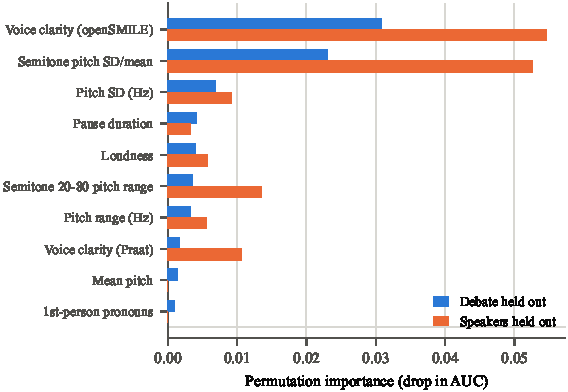
\includegraphics[width=\columnwidth]{figures/fig_rf_importance.pdf}
  \caption{Permutation importance of the top ten measures. The ranking is
  almost entirely acoustic, and it is led by the two measures shown in
  Section~\ref{sec:method:acoustic} to be tied to the speaker's own voice.}
  \label{fig:rf}
\end{figure}

Table~\ref{tab:forest} and Figure~\ref{fig:rf} show that nine of the top ten
measures are acoustic under either holdout scheme. The best text measure
contributes about three per cent of what the top acoustic measure does. The
forest leans hardest on the two measures already shown to be compromised:
voice clarity and semitone pitch variation, both tied to the speaker's own
voice (Section~\ref{sec:method:acoustic}). The measure that survives every
validity check ranks only sixth. The ranking barely changes when speakers
are held out. What changes, in the next section, is whether the
ranking is worth anything.

\subsection{Debate Held Out Versus Speakers Held Out}
\label{sec:method:heldout}

We use the same random forest and the same two holdout schemes to answer the
practical question directly: given a sentence, or a whole debate, how often
can a model say which candidate went on to win?

Alongside accuracy, Table~\ref{tab:accuracy} reports the area under the
curve (AUC). AUC has a direct reading: take one sentence from a winning
candidate and one from a non-winning candidate, both at random, and AUC is
the probability the model scores the winning one higher. A model that has
learned nothing scores $0.5$; one that always gets the pair right scores
$1.0$. Unlike accuracy, AUC does not depend on group sizes, which matters
here because the two outcome groups are unequal in size. $0.5$ is the
right baseline only when the held-out items are independent, a condition
that fails for twelve of the fourteen speaker folds below, which is why we
also report the paired debate-level test later in this section.

\begin{table}[t]
\caption{How often the forest identifies the winning candidate. Always
guessing the larger group scores $0.530$.}
\label{tab:accuracy}
\centering
\footnotesize
\setlength{\tabcolsep}{4pt}
\begin{tabular}{lrr}
\toprule
 & Debate & Speakers \\
 & held out & held out \\
\midrule
\multicolumn{3}{l}{\emph{Sentence level} ($23{,}082$ sentences)} \\
Accuracy               & $0.596$ & $0.518$ \\
Area under curve       & $0.630$ & $0.523$ \\
\midrule
\multicolumn{3}{l}{\emph{Debate level} ($24$ debates)} \\
Debates called correctly & $17/24$ & $12/24$ \\
$p$ against a coin       & $0.064$ & $1.00$ \\
\midrule
Majority-class baseline  & \multicolumn{2}{c}{$0.530$} \\
\bottomrule
\end{tabular}
\end{table}

Table~\ref{tab:accuracy} shows that with the debate held out, sentence
accuracy is $0.596$ against a $0.530$ baseline. Debate-level calls are
$17/24$, not significant against a coin ($p = 0.064$). With the speakers
held out, sentence accuracy falls to $0.518$, \emph{below} the
majority-class baseline. Debate-level calls are $12/24$, an exact coin
flip. Errors stay symmetric under speaker holdout (precision/recall near
$0.49$/$0.54$ either way), which indicates an uninformative model rather
than a biased one.

The natural test of speaker generalisation is to hold out a speaker,
predict their sentences, and score the result. That test cannot be run
directly here. Twelve of fourteen speakers appear in only one outcome
class, so within those folds there is only one class to discriminate, and
the area under the curve is undefined. Pooling scores across folds is also
not valid, since that would compare differently-calibrated models rather
than measuring discrimination within any one of them. The valid test is
paired and within debate: for each debate, does the winning candidate's
mean score beat the opponent's? Both classes are present by construction
and both are scored by the same model.

\begin{table}[t]
\caption{The paired test. For each debate, did the winning candidate's mean
score beat the opponent's?}
\label{tab:paired}
\centering
\footnotesize
\begin{tabular}{llrr}
\toprule
Model & Held out & Debates & $p$ \\
\midrule
\multirow{2}{*}{Weighted sum}    & debate only   & $17/24$ & $0.064$ \\
                                 & both speakers & $11/24$ & $0.84$ \\
\multirow{2}{*}{Discriminant} & debate only    & $19/24$ & $0.0066$ \\
                              & both speakers  & $10/24$ & $0.54$ \\
\multirow{2}{*}{Decision forest} & debate only   & $17/24$ & $0.064$ \\
                                 & both speakers & $12/24$ & $1.00$ \\
\bottomrule
\end{tabular}
\end{table}

\begin{figure}[t]
  \centering
  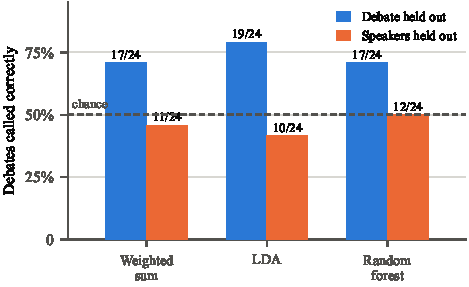
\includegraphics[width=\columnwidth]{figures/fig_holdout.pdf}
  \caption{The same three methods, evaluated two ways. Holding out the debate
  leaves both of its speakers in the training data; holding out the speakers
  removes them entirely. All three fall to chance under the stricter test.}
  \label{fig:holdout}
\end{figure}

Table~\ref{tab:paired} and Figure~\ref{fig:holdout} give the cleanest
result in the paper. Holding out only the debate, the discriminant calls
$19$ of $24$ correctly ($p = 0.0066$). The weighted sum and forest each call
$17$ of $24$ correctly ($p = 0.064$). Holding out the speakers as well, the
discriminant falls to $10/24$, the forest to $12/24$, and the weighted sum
to $11/24$. Three methods, three different assumptions about the shape of
the data, one result: what looked like a model of how winners speak was a
model of who the winners were.

\subsection{Predictive Association Versus Recurrence}
\label{sec:method:recurrence}

\begin{table}[t]
\caption{Repeatability. ``Dir.'' is debates in the same direction out of $24$.
$I^2$ is the percentage of variation between debates rather than sampling
noise. LOSO is the range when each speaker in turn is dropped. PI is the
prediction interval for a new debate.}
\label{tab:grid}
\centering
\scriptsize
\setlength{\tabcolsep}{2pt}
\begin{tabular}{lrrrrr}
\toprule
Measure & Eff. & Dir. & $I^2$ & LOSO & PI \\
\midrule
Semitone 20--80 range & $-0.226$ & $21/24$ & $94$ & $[-.31,-.17]$ & $(-.81,+.32)$ \\
Semitone SD/mean      & $-0.332$ & $20/24$ & $96$ & $[-.44,-.27]$ & $(-1.10,+.36)$ \\
Declination-resid.\ SD & $-0.242$ & $20/24$ & $96$ & stable       & $(-.98,+.45)$ \\
Adjective rate        & $+0.062$ & $17/24$ & $59$ & stable        & $(-.10,+.23)$ \\
Voice clarity (A)     & $+0.461$ & $13/24$ & $99$ & ---           & $(-1.61,+2.80)$ \\
Voice clarity (B)     & $+0.315$ & $13/24$ & $99$ & $[+.11,+.47]$ & $(-1.51,+2.28)$ \\
Pitch variation (Hz)  & $-0.228$ & $17/24$ & $98$ & $[-.37,-.16]$ & $(-1.17,+.67)$ \\
Pause proportion      & $+0.196$ & $14/24$ & $98$ & sign flips    & $(-.79,+1.03)$ \\
Articulation (syll/s) & $+0.108$ & $17/24$ & $96$ & stable        & $(-.59,+.86)$ \\
Sentiment polarity    & $+0.030$ & $17/24$ & $74$ & stable        & $(-.20,+.26)$ \\
\bottomrule
\end{tabular}
\end{table}

\textbf{Every prediction interval in Table~\ref{tab:grid} includes zero},
for every measure that survived every check up to this point. A difference
can satisfy all of the following: it can be present across the whole
corpus, statistically significant within debates, visible in $20$ or $21$
debates out of $24$, and pass every check in Section~\ref{sec:method:validity}.
Even so, it can still tell us nothing about the twenty-fifth debate. One
objection deserves an answer: perhaps $24$ debates simply cannot produce a
prediction interval that excludes zero. Adjective rate answers it: its
between-debate variation is low ($I^2 = 59\%$), and its interval,
$(-0.10, +0.23)$, is within a factor of two of clearing. The
obstacle is inconsistency between debates, not sample size. Between $59\%$
and $99.5\%$ of the variation in these measures is between debates rather
than between candidates.

\subsection{Exploratory Same-Candidate Analysis}
\label{sec:method:samecand}

Only two candidates were observed both winning and losing a general
election. We fit the discriminant with each entirely removed, then project
their debates into the space. For George H.\,W.\ Bush, the separation is
complete: every debate he won scores above every debate he lost, and the
model never saw him during fitting ($6/6$; gap $+0.173$). For Donald Trump
the gap is $+0.005$, essentially nothing ($4/6$). One speaker's winning and
losing debates are also four years apart. The standardisation controls for
that time period, but not for anything else that changed in the interim.
Two cases cannot settle the exploratory question posed in
Section~\ref{sec:intro:rq}. We report them because they are the only direct
evidence the corpus contains. Full debate-by-debate scores are in
Appendix~\ref{app:samecand}.

The textbook remedy for sentences nested inside speakers is a random
effect per speaker. That remedy cannot be estimated here. Regressing the
outcome label on speaker identity across the $51$ candidate-by-debate cells
gives $R^2 = 0.811$: \textbf{speaker identity explains $81\%$ of whether a
candidate won}. Twelve of fourteen speakers appear in one outcome class
only, so for them the two variables are the same variable. As a result, the
variance of the outcome coefficient is inflated $5.3$-fold, and only $36$
residual degrees of freedom remain. A speaker random effect would not make
the analysis better powered here. It would make it better calibrated. The
honest output of a correctly calibrated model on this corpus is a very wide
interval.

Section~\ref{sec:method:llmprotocol} gives the protocol for testing a large
language model on the same question. What follows is the result, reached
independently of the three classical models above.

\subsection{Transcript-Only and Descriptor-Only Judgments}
\label{sec:method:llm}
\label{sec:llm:accuracy}

\begin{table}[t]
\caption{The language model's debate-level accuracy (majority vote over $3$
re-randomised repeats) beside how often a separate, question-free probe
identifies the actual debate from the same input.}
\label{tab:crossmodal}
\centering
\footnotesize
\setlength{\tabcolsep}{4pt}
\begin{tabular}{lrr}
\toprule
Input             & Outcome accuracy & Exact debate identified \\
\midrule
Descriptors only  & $13/24$          & $0/24$ \\
Transcript only   & $24/24$          & $24/24$ \\
\bottomrule
\end{tabular}
\end{table}

Given the anonymised transcript, the model calls the winner in $24$ of $24$
debates. Given only the descriptor table, with no text, it calls $13$ of
$24$, a coin flip ($p = 0.340$). Read alone, the first number looks like the
model successfully reasoning over communicative style from text.
Section~\ref{sec:llm:contamination} shows that it is not.

\subsection{Contamination Probe}
\label{sec:llm:contamination}

We give the same model the same anonymised transcript with no prediction
question attached, and ask it to name the debate. It names the specific
real debate---year and both candidates---in $24$ of $24$ cases
(Table~\ref{tab:crossmodal}). Given the descriptor table alone, it does so
in $0$ of $24$. Presidential debate transcripts are some of the most quoted
text in existence. Stripping names and dates removes the labels, but it
does not remove lines like ``I did not have sexual relations with that
woman,'' or a candidate saying ``you're likable enough, Hillary.''
\textbf{The language model's transcript-based accuracy cannot be
interpreted as evidence of generalisable political-language reasoning,
because the model identifies the exact debate from the same anonymised
input in every case.} This is the same failure mode
Section~\ref{sec:method:heldout} found in the decision forest and the
discriminant, though arrived at here by a completely different method. What
looks like the modality that helps is the modality that leaks identity.

\begin{figure}[t]
  \centering
  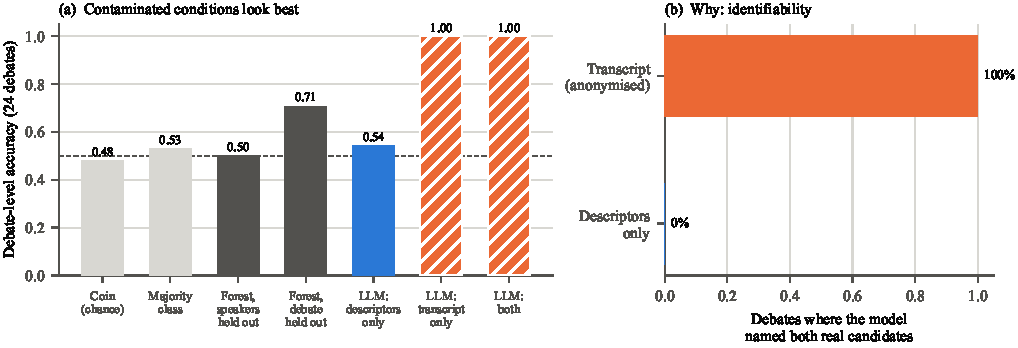
\includegraphics[width=\columnwidth]{figures/fig_crossmodal.pdf}
  \caption{(a) Debate-level accuracy of the language model, against the
  decision forest and the trivial baselines. The transcript condition
  (hatched) beats everything else in the paper. (b) shows why: the same
  model, asked only to identify the debate rather than predict its outcome,
  does so perfectly whenever it can see the transcript, and never when it
  can only see numbers.}
  \label{fig:crossmodal}
\end{figure}

Figure~\ref{fig:crossmodal} places the two results side by side. This is
also the direct answer to a concern raised in Section~\ref{sec:intro:gaps}
and revisited in Section~\ref{sec:concl:future}: whether a language model can
identify a debate and its outcome from anonymised material is a number to
report, not a caveat to mention. Here, it is $100\%$ for text and $0\%$ for
numbers.

\subsection{Grounding of Explanations}
\label{sec:llm:grounding}

Every prediction call also cites, from a closed vocabulary, which evidence
it relied on. This lets us check the citations by machine against the real
data instead of taking them on faith. Given descriptors and citing a
specific measure, the citation points the right way $75.8\%$ of the time
($303/400$ citations). With the transcript added, this rises to $84.3\%$
($348/413$). Read alone, the second number looks like better reasoning with
more evidence. Read alongside the contamination result, a less flattering
explanation fits at least as well. Once the transcript has told the model
who wins, a numeric citation only has to sound consistent with an answer
already fixed, not actually justify it. In the descriptors-only condition,
where no such shortcut exists, the model's most-cited measures are
loudness, sentence length, voice clarity, grade level and speech rate. Its
explanations read as plausible performance narratives, such as this one:
``\emph{Candidate B shows higher pitch variability, faster articulation
rate, and more syntactically complex speech\ldots which suggests a more
dynamic and sophisticated delivery}''. This call was made in the $1988$
debate, for a candidate who went on to lose. Every one of those measures
was already found, in Section~\ref{sec:method:forest} or
Appendix~\ref{app:supplement}, to be uncorrelated with winning or confounded
with it. A fluent explanation is not the same thing as a correct one. We
scan the transcript-only explanations for invented acoustic numbers,
meaning any figure the model was never given. We find none in any of the
$72$ transcript-condition responses. On this specific, narrow check, the
model does not fabricate.

\subsection{Implications for LLM-as-Judge Research}
\label{sec:llm:implications}

Evaluating a language model's judgment of famous political material needs
at least two controls beyond accuracy: an identification or contamination
probe, asked with no task question attached, and a check that cited reasons
are actually consistent with the evidence presented rather than merely
fluent. Neither control is specific to debates or to this model, and both
are cheap to run. Section~\ref{sec:disc:llm} returns to what they generalise
to.

%=======================================================================
\section{Discussion}
\label{sec:disc}
%=======================================================================

\subsection{What Differs Between Eventual Winners and Non-Winners}
\label{sec:disc:whatdiffers}

Across four levels and $53$ properties, we find no robust broad linguistic,
semantic or discourse-level separation between the two groups
(Sections~\ref{sec:method:linguistic}--\ref{sec:method:discourse}). We find
one coherent pitch-control family. Within it, one measure,
declination-residual standard deviation, is the
strongest measurement-valid result in the paper (Section~\ref{sec:method:pitch}). The
two original broad-screen pitch measures and this one describe the same
underlying phenomenon at increasing precision: less overall range, less
range relative to habitual pitch, and, most specifically, less local
movement once each sentence's own trend is removed.

The text-based comparison illustrates why we insist on that precision. The
pooled, uncontrolled profile of Section~\ref{sec:data:descriptive} and the
within-debate screen of Section~\ref{sec:method:linguistic} are the same
comparison: one candidate group against the other. They are run at two
different levels of control, and they do not always agree. Adjective rate points the
same way at both levels (higher among winning candidates, pooled and
within-debate alike) without ever surviving correction. Third-person
pronoun rate flips sign between the two. Pooled, winning candidates use it
less. Within debates, the difference is indistinguishable from zero, in the
other direction. The discourse-tag frequencies of
Table~\ref{tab:tagdiff} point the same way as the pooled text
measures. Section~\ref{sec:method:discourse} shows why we do not trust
them either: several of the largest pooled differences come from detectors
that fire on a single string. None of this changes what Section~\ref{sec:method:pitch}
finds. It is why we report a naive comparison at all, rather than only the
validated one that survives correction.

\subsection{Interpretation of Residual Pitch Stability}
\label{sec:disc:mechanism}

This analysis establishes a correlation between electoral outcome and one
specific property of a pitch contour. It does not establish why that
property might matter to a listener. We ran no perception experiment to
find out. What follows is a plausible account, built from findings already
cited in this paper. We offer it as interpretation rather than result.

Two production-side mechanisms and one perception-side mechanism point the
same way. On the production side, planning an utterance in advance and
executing it as one coherent unit is understood to produce a single, matched
intonational gesture. Formulating a sentence while speaking it---as when a speaker reformulates a
claim mid-sentence, hedges, or searches for the next word---is understood to
introduce small disruptions to that gesture, as the plan is revised in real
time \cite{levelt1989speaking}. A rehearsed answer and an
improvised one are not expected to look the same on this measure. Debate
answers are frequently at least partly rehearsed in advance.
Separately, fine control over the laryngeal muscles that set pitch is
understood to be sensitive to physiological effort and strain. Steadier
voluntary control produces a cleaner pitch trajectory, and reduced control
introduces the kind of small involuntary fluctuation this measure is built
to detect \cite{laver1980voice}. On the perception side, the same
voice-quality literature treats predictable, steady prosody as a standing
cue to fluency and confidence, largely independent of what is being said
\cite{laver1980voice}. If any of these mechanisms is operating here, a
listener would not need to consciously notice the pitch contour to be
influenced by it.

This interpretation connects directly to the factorial design we propose in
Section~\ref{sec:concl:future}. That design pairs independently manipulated
text and prosody with listener ratings. A declination-residual measure
computed on the resynthesised audio in that design would test directly
whether steadier residual pitch movement raises a listener's rating of
vocal control, holding the words fixed. Nothing in the present corpus can
adjudicate between the mechanisms above, or confirm that any one of them is
operating rather than some fourth explanation. The corpus establishes only
that the acoustic pattern exists and is not an artefact of speaker identity,
sentence length, or transcription treatment.

\subsection{Speaker Identity Versus ``Winning Style''}
\label{sec:disc:identity}

Twenty-four thousand candidate sentences do not equal $24{,}193$ independent
outcome observations. They come from fourteen people. Any
generalisation claim has to hold up over those fourteen people, not over
the sentence count. Holding out a debate while leaving its speakers' other
debates in training (Section~\ref{sec:method:heldout}) is not a held-out
test of speaker identity. The gap between the two holdout schemes---$19/24$
to $10/24$ for the discriminant, $17/24$ to $12/24$ for the forest, $17/24$
to $11/24$ for the weighted sum---is the size of that confound made
visible. Feature stability under permutation importance
(Table~\ref{tab:forest}) does not imply transferable prediction. The same
top-ranked measures survive speaker holdout, but the forest's ability to
use them does not.

\subsection{What the Null Results Contribute}
\label{sec:disc:nulls}

The null findings sharpen rather than weaken the positive one. Not
sentiment. Not pronoun use, at any grammatical person. Not general
syntactic complexity. Not pitch velocity, acceleration, or how often the
pitch contour changes direction. Not most rhetorical categories, once we
check the detectors that claimed to measure them. What remains after this
many specific nulls is not ``pitch matters, vaguely.'' It is one measurable
property of one signal. It is characterised precisely enough that a null result
on a neighbouring measure (turning-point rate; kurtosis) rules out specific
alternative explanations rather than merely failing to reach significance.

\subsection{Implications for Multimodal Modelling}
\label{sec:disc:multimodal}

This lesson extends past presidential debates. A multimodal system trained
on a small, repeatedly-observed population of subjects can improve its
apparent performance by exploiting identity-bearing information, acoustic
or textual, rather than the task-relevant behaviour it was meant to
capture. Debate-level holdout alone will not reveal this if the same
individuals recur across the held-out and training partitions. Three
structurally different models (Section~\ref{sec:method:generalise}) reach
this failure mode independently. A fourth, a large language model
(Section~\ref{sec:method:llm}), reaches the text-modality version of the
same failure by a completely different route.

\subsection{Implications for LLM Research}
\label{sec:disc:llm}

Memorisation of famous transcripts is not a remote risk for
language-model evaluation on any well-known text. It is directly
measurable with a question-free identification probe. Here it was
total for the raw transcript and absent for numeric descriptors of the same
material. Partial anonymisation (names, party and dates removed, content
untouched) was sufficient to demonstrate the contamination without
destroying the communicative content the transcript condition existed to
test. It was not sufficient to prevent the contamination itself. That
is the more important number to report. A grounding
requirement---citations checkable against real data, from a closed
vocabulary---separates answer accuracy from valid reasoning in a way
free-text explanation cannot. We treat it as a minimum bar for
LLM-as-judge use on any material a model may have seen before, not only on
debate transcripts.

\subsection{Relationship to Previous Research}
\label{sec:disc:relationship}

Rosenberg and Hirschberg's \cite{rosenberg2009acoustic} expectation that
pitch and pausing would matter most is broadly supported. The only
broad-screen measures that survive are pitch measures. The pausing
result does not survive the speaker check, but the effect is large enough
that it would have looked like a genuine finding without that check. K\"unzel's
\cite{kunzel1989speakers} warning about average pitch is directly borne out
by the paper's largest and least trustworthy effect (voice clarity,
Section~\ref{sec:method:acoustic}). What this design adds, that a
single-cycle or single-debate study could not, is the speaker-aware
evaluation that turns ``pitch range differs'' into ``pitch range differs,
and specifically the residual component of it, in a way that does not yet
predict an unseen debate.'' This is a more qualified conclusion than the
charisma literature's framing, and we take it to be a more useful one.

%=======================================================================
\section{Limitations and Future Work}
\label{sec:concl:limits}
%=======================================================================

\subsection{Corpus Limitations}
\begin{itemize}\itemsep2pt
  \item \textbf{Fourteen speakers is few.} Nine elections and fourteen
        people can reveal only differences that are nearly universal. A
        null result means no evidence, not evidence of nothing.
  \item \textbf{Third-party candidates are not like major-party losers.}
        Ross Perot contributes $1{,}024$ sentences. Dropping him and
        recomputing is the only evidence we have on how much he matters.
  \item \textbf{One language, one broadcasting tradition.}
  \item \textbf{Two 2024 debates are excluded} for unverifiable speaker
        attribution (Appendix~\ref{app:known}). Including them changes
        several secondary results and none of the primary ones.
\end{itemize}

\subsection{Measurement Limitations}
\begin{itemize}\itemsep2pt
  \item \textbf{Some timings are interpolated.} Missing acoustic data
        is uneven across alignment treatments ($2.8\%$ against $16.5\%$).
  \item \textbf{Interruptions are not represented.} No two candidate
        sentences overlap in time, including in the 2020 debate, which was
        defined by people talking over each other.
  \item \textbf{Sentence boundaries vary across the corpus.} Every
        per-sentence count depends on them.
  \item \textbf{A quarter of sentences are too short} for reliable voice
        measurement (Table~\ref{tab:reliab}).
\end{itemize}

\subsection{Inferential Limitations}
\begin{itemize}\itemsep2pt
  \item \textbf{The election result is not a measure of good speaking.} It
        is a shared external target. No claim here depends on winning
        and speaking well being the same thing.
  \item \textbf{This is correlation.} Winners differ from losers in
        incumbency, money, party position and prior office. Incumbency can
        be added within debates at no cost and should be the first control
        a follow-up adds.
  \item \textbf{Every prediction interval reported includes zero.} An
        association can be real, significant, and repeatedly observed
        across this corpus without yet supporting a prediction about a
        debate we have not seen (Section~\ref{sec:method:recurrence}).
\end{itemize}

\subsection{LLM Limitations}
\begin{itemize}\itemsep2pt
  \item \textbf{One model, one API version, one evaluation date.} Every
        language-model result in this paper uses \texttt{claude-opus-4-8}
        on $2026$-$08$-$06$ (Appendix~\ref{app:llmrepro}). We tested one
        prompting variation (chain-of-thought against direct). It made
        no difference, but we cannot rule out that a different model or
        prompt would.
  \item \textbf{The training-data concern is measured, not assumed.} The
        contamination probe (Section~\ref{sec:llm:contamination}) shows the
        model identifies the exact debate, year and both candidates from an
        anonymised transcript in $24$ of $24$ cases. This corpus cannot be
        absent from the training data. Its memorisation is directly
        measurable. Any result touching the transcript text has to be
        read through that fact.
  \item \textbf{Discourse-tag agreement here is instrument-versus-instrument,
        not instrument-versus-ground-truth.} We compare rule-based and
        model-based labels against each other
        (Section~\ref{sec:method:discourse}). Neither is validated against
        adjudicated human judgment. The chance-level agreement on
        rhetorical categories is informative about the instruments'
        disagreement with each other, not proof that either is wrong.
\end{itemize}

\subsection{Future Work}
\label{sec:concl:future}

Two studies would extend this design most directly: an expanded
observational corpus, and a controlled experiment that manipulates text and
prosody independently.

\emph{An expanded observational corpus.} The limit on the substantive
question is the number of elections, not the amount of speech. Adding
vice-presidential, primary, senatorial and gubernatorial debates would keep
the format while multiplying the speakers and the contested outcomes. It
would also supply many more people who both win and lose. Every check reported
here carries over unchanged.

\emph{A controlled text$\times$prosody perception experiment.} In observed
speech, what a candidate says and how they say it always arrive together
from the same person, which is why no corpus of this kind can separate
them. We propose the following design instead. Take an utterance. Rewrite
the words with a language model to be more or less charismatic, holding
content fixed. Resynthesise the delivery, holding words fixed. Cross the two
so each utterance appears in four versions. Then have listeners rate vocal
control, confidence, charisma, credibility and persuasiveness:
\begin{equation}
\begin{split}
C \;=\; \beta_0 &+ \beta_1(\text{text}) + \beta_2(\text{prosody}) \\
                &+ \beta_3(\text{text} \times \text{prosody}) \\
                &+ u_{\text{speaker}} + u_{\text{listener}} + \varepsilon .
\end{split}
\label{eq:factorial}
\end{equation}
Now $\beta_1$ and $\beta_2$ are separately identified, because the
experimenter assigned them rather than the candidate. Both random
effects are estimable, because every speaker and listener appears in every
condition, a property this corpus lacks. Language models can rewrite text
while holding content roughly fixed. Current speech synthesis allows
independent control of pitch, energy, rate and style. Together, these make
this design practical now.

Two cautions carry over from this paper. The first is no longer
hypothetical. Section~\ref{sec:llm:contamination}'s contamination probe
confirms directly that a language model given an anonymised transcript from
this corpus identifies the debate in every case. The same check has to run
on whatever text a language model rewrites for the design above, and on the
rewritten output itself. It must run before any listener sees the material,
not only on the original transcript. Numeric descriptors did not carry the
same signal in our check. Rewritten, resynthesised speech, however, is a
different object again, and it should not be assumed clean until tested.
The second caution is more straightforward: these are fourteen of the most
recognisable voices in America, so listeners will identify them. Whether a
listener recognised the speaker should be recorded and modelled, not assumed
away.

%=======================================================================
\section{Conclusion}
\label{sec:concl}
%=======================================================================

In this paper we describe a multimodal analysis of every televised U.S.\
general-election presidential debate from 1988 to 2020. We first compare
candidate speech with a pooled, uncontrolled text-based profile. Several of
its differences (adjective rate, third-person pronoun rate, patriotic and
historical rhetorical framing) shrink, disappear or reverse once the same
comparison is repeated within debates. For the discourse categories, they
also shrink, disappear or reverse once the detectors producing them are
audited. We then screen
$43$ linguistic, semantic, discourse and acoustic measures for a
within-debate difference between eventual winning and non-winning
candidates. We follow the one acoustic property that survives down to the
level of the pitch contour itself. We find that eventual winning candidates
show less residual
pitch movement than eventual non-winning candidates, once each sentence's
own broad rise or fall is removed. The effect is $-0.242$ standard deviations,
present in $20$ of $24$ debates, stable across fourteen
leave-one-speaker-out refits, uncoupled from habitual pitch, and, unlike a
measurement artefact, stronger rather than weaker in longer sentences. Of
$53$ properties measured at four levels, this is the one pattern that
survives every check we ran.

We demonstrate, however, that this association does not yet support
reliable prediction for an unseen speaker or a new debate: its $95\%$
prediction interval includes zero, for a structural reason rather than a
statistical one. Only fourteen people have ever taken this stage, and twelve of
them did so only once. Speaker identity explains $81\%$ of the outcome label those
fourteen people carry.

We show that this same structural fact is why a decision forest, a linear
discriminant, a weighted sum, and a large language model all appeared, at
first pass, to predict the winner. It is also why all four stopped working
once we changed the evaluation to remove speaker or transcript identity,
rather than merely the debate under test. We conclude that speaker-aware
validation---holding out every debate a candidate ever appears in, not just
the one under test---and, for a language model, a question-free
contamination probe alongside a closed-vocabulary grounding check, are not
optional refinements to this kind of analysis. They are the difference
between a predictive result and an artefact of who, or what text, the model
had already seen.

The advantage of the speaker-aware and contamination-aware protocol used
throughout this paper is that it is cheap to apply and specific to no one
model: the same two holdout schemes and the same two language-model checks
generalise to any multimodal study of a small, repeatedly-observed
population of speakers. Limitations of the present corpus and directions
for extending it are given in Section~\ref{sec:concl:limits}.

\section*{Acknowledgments}
The author thanks the maintainers of the open-source speech and language tools
on which this work depends.

%=======================================================================
\begin{appendices}
%=======================================================================

\section{Debate Inventory}
\label{app:inventory}

\begin{table}[h]
\caption{Every debate in the corpus: date, candidates, and which ticket won
the election that followed. Audio and official transcripts are cited by
debate identifier in the deposited data statement (Appendix~\ref{app:resource}).}
\label{tab:inventory}
\centering
\scriptsize
\setlength{\tabcolsep}{2pt}
\begin{tabular}{llp{0.42\columnwidth}l}
\toprule
ID & Date & Candidates & Winner \\
\midrule
1001 & 1988-09-25 & G.\,H.\,W.\ Bush vs.\ Dukakis & Bush \\
1003 & 1988-10-13 & G.\,H.\,W.\ Bush vs.\ Dukakis & Bush \\
1004 & 1992-10-11 & Clinton vs.\ Perot, G.\,H.\,W.\ Bush & Clinton \\
1006 & 1992-10-15 & Clinton vs.\ Perot, G.\,H.\,W.\ Bush & Clinton \\
1007 & 1992-10-19 & Clinton vs.\ G.\,H.\,W.\ Bush, Perot & Clinton \\
1008 & 1996-10-06 & Clinton vs.\ Dole & Clinton \\
1010 & 1996-10-16 & Clinton vs.\ Dole & Clinton \\
1011 & 2000-10-03 & G.\,W.\ Bush vs.\ Gore & Bush \\
1013 & 2000-10-11 & G.\,W.\ Bush vs.\ Gore & Bush \\
1014 & 2000-10-17 & G.\,W.\ Bush vs.\ Gore & Bush \\
1015 & 2004-09-30 & G.\,W.\ Bush vs.\ Kerry & Bush \\
1017 & 2004-10-08 & G.\,W.\ Bush vs.\ Kerry & Bush \\
1018 & 2004-10-13 & G.\,W.\ Bush vs.\ Kerry & Bush \\
1019 & 2008-09-26 & Obama vs.\ McCain & Obama \\
1021 & 2008-10-07 & Obama vs.\ McCain & Obama \\
1022 & 2008-10-15 & Obama vs.\ McCain & Obama \\
1023 & 2012-10-03 & Obama vs.\ Romney & Obama \\
1025 & 2012-10-16 & Obama vs.\ Romney & Obama \\
1026 & 2012-10-22 & Obama vs.\ Romney & Obama \\
1027 & 2016-09-26 & Trump vs.\ H.\ Clinton & Trump \\
1029 & 2016-10-09 & Trump vs.\ H.\ Clinton & Trump \\
1030 & 2016-10-19 & Trump vs.\ H.\ Clinton & Trump \\
1031 & 2020-09-29 & Biden vs.\ Trump & Biden \\
1033 & 2020-10-22 & Biden vs.\ Trump & Biden \\
\bottomrule
\end{tabular}
\end{table}

\section{Alignment and Preprocessing}
\label{app:align}

Audio was converted to single-channel PCM at $16$~kHz. For matching, both the
recognised text and the official transcript were reduced to lower-case
alphanumeric tokens. Punctuation was removed, contractions were left
unexpanded, and numerals were kept as written. The match rate is the share
of official-transcript tokens that fall inside a matching block. Matching
blocks were found with a longest-matching-block algorithm. Routing
thresholds were $\geq 85\%$ and $60$--$85\%$.

Recognition used Whisper \cite{radford2023whisper}, which gives word-level
timings. Matched tokens take those timings directly. Unmatched runs are
interpolated between the nearest matched words, split by character count.

Montreal Forced Aligner \cite{mcauliffe2017mfa} was run with the English ARPA
acoustic model and dictionary. Default beam settings did not finish on
ninety-minute recordings, so production runs used wider beams under a
watchdog. It converged on $20$ of $24$ debates and is kept as an independent
check.

\section{Complete Feature Definitions}
\label{app:features}
\label{app:tools}

Pitch, loudness and voice-quality measures come from Praat
\cite{boersma2024praat} through \texttt{parselmouth}. The $88$-parameter set
comes from openSMILE \cite{eyben2010opensmile,eyben2016gemaps}, which also
supplies the semitone pitch measures and the second voice-clarity
implementation. Parsing and tagging use spaCy \cite{honnibal2020spacy} with
\texttt{en\_core\_web\_sm}, the smallest available model. Its weakest
outputs are parse depth and dependency length. Sentiment uses VADER
\cite{hutto2014vader}, topic categories use Empath \cite{fast2016empath}, and
sentence vectors use Sentence-BERT \cite{reimers2019sbert}.

A silent pause is a stretch of at least $150$~ms during which loudness stays
at least $25$~dB below the ninetieth percentile for that sentence. The usual
threshold after Goldman-Eisler \cite{goldman1968psycholinguistics} is
$250$~ms. The detector cannot see filled pauses. Whether those were
transcribed at all varies across this corpus.

Table~\ref{tab:featuredict} names the $34$ standardised measures used in
Sections~\ref{sec:method:combined} and~\ref{sec:method:llmprotocol}. These
overlap heavily with the full $43$-measure broad screen
(Section~\ref{sec:method:measures}). The remaining measures are named
individually in the results prose of Section~\ref{sec:method:screen}:
jitter, shimmer, four readability scores, positive/negative sentiment, and
the $35$ topic categories, which are treated as one diagnostic family
rather than as individual screened measures.

\begin{table}[h]
\caption{The $34$ standardised measures used in the combined and LLM
analyses, by family.}
\label{tab:featuredict}
\centering
\scriptsize
\setlength{\tabcolsep}{2pt}
\begin{tabular}{p{0.30\columnwidth}p{0.30\columnwidth}p{0.30\columnwidth}}
\toprule
Acoustic (Praat) & Acoustic (openSMILE) & Linguistic \\
\midrule
Mean pitch & Syllable rate & Clauses \\
Pitch SD (Hz) & Articulation rate (syll/s) & Subordinate clauses \\
Pitch range (Hz) & Semitone pitch SD/mean & Parse depth \\
Loudness & Semitone $20$--$80$ range & Dependency length \\
Voice clarity (Praat) & Voice clarity (openSMILE) & Words per sentence \\
Pause duration & & Word length \\
Pause count & & Function words \\
Mean pause length & & 1st/2nd/3rd-person pronouns \\
Speech rate & & Nouns, verbs, adjectives, adverbs \\
Articulation rate (w/s) & & Reading ease, grade level \\
 & & Sentiment, positive, negative \\
\bottomrule
\end{tabular}
\end{table}

For the frame-level pitch-contour measures (Section~\ref{sec:method:pitch:extract}),
the low-level-descriptor output of openSMILE
(\texttt{F0semitoneFrom27.5Hz\_sma3nz}, $10$~ms hop) was run independently
per sentence clip. We first tried slicing these measures from a
continuously smoothed whole-debate stream, but rejected this approach:
continuous smoothing across sentence boundaries shifted the resulting
statistics measurably at clip edges. Distributional measures use all
voiced frames regardless of order. Dynamic measures use only differences
between temporally consecutive voiced frames. Declination slope and its
residual standard deviation come from an ordinary-least-squares fit of the
semitone contour against frame time.

Four measurement problems are recorded for anyone reusing the corpus.
\emph{One pitch range for everyone}: the analysis range was $75$--$500$~Hz
for a corpus where average pitch runs from $102.5$ to $195.9$~Hz. The
fixed $75$~Hz floor is the likely cause of the pitch-dependence of voice
clarity. \emph{Mismatched floors}: Praat's loudness default assumes a
minimum pitch of $100$~Hz against the $75$~Hz used for pitch. \emph{Voiced
fraction} runs from $0.583$ to $0.742$ across speakers. It correlates with
voice clarity at $+0.674$ at speaker level, and this relationship persists
within a single speaker in a single debate, at a median of $+0.327$. \emph{Reliability
depends steeply on sentence length} (Table~\ref{tab:reliab}), which is why
the length check in Section~\ref{sec:method:acoustic} had to be run first.

\begin{table}[h]
\caption{Voice-clarity reliability by sentence length. Split-half reliability
is odd-versus-even sentences within one speaker in one debate.}
\label{tab:reliab}
\centering
\begin{tabular}{lrrr}
\toprule
Sentence length & Mean clarity & SD & Split-half \\
\midrule
$0.3$--$1.0$~s  & $8.79$~dB  & $3.10$ & $0.126$ \\
$1.0$--$2.5$~s  & $9.51$~dB  & $2.42$ & $0.476$ \\
$2.5$--$6.0$~s  & $9.96$~dB  & $2.16$ & $0.655$ \\
$6.0$~s$+$      & $10.30$~dB & $2.00$ & $0.729$ \\
\midrule
\multicolumn{4}{l}{Candidate sentences: median $3.02$~s, IQR} \\
\multicolumn{4}{l}{$(1.53, 5.71)$; $24.2\%$ under $1.5$~s, $13.1\%$} \\
\multicolumn{4}{l}{under $1.0$~s, $4.6\%$ under $0.5$~s.} \\
\bottomrule
\end{tabular}
\end{table}

\section{Full Statistical Results}
\label{app:stats}

Debate effects are removed by subtracting each debate's mean. Cluster-robust
variances use a sandwich estimator with a small-sample correction. These are
referred to a $t$ distribution with $G-1$ degrees of freedom: $G = 24$ for
debate clustering and $14$ for speaker clustering. With this few clusters
the $p$-values should be read as generous rather than exact.

The randomization test enumerates all $2^{24} = 16{,}777{,}216$ ways of
flipping the winner label within debates. Random-effects pooling follows
DerSimonian--Laird. The prediction interval is computed as the pooled
estimate $\pm\, t_{22}\sqrt{\tau^2 + \mathrm{SE}^2}$. Leave-one-speaker-out
recomputes the within-debate effect with one speaker's sentences removed.

Several of the $43$ measures overlap: $13$ pairs correlate above $|r| =
0.7$. The effective number of independent measures is $30.0$ by the Li--Ji
method. Correcting at $m = 30$ instead of $m = 43$ changes nothing.

Section~\ref{sec:method:heldout} defines the area under the curve (AUC)
reported for the discriminant and forest, and explains why $0.5$ is the
right baseline only when the held-out items are independent.

The deposited version of this appendix carries the full table over all $43$
measures, the treatment-split table, and all $35$ topic categories.

\section{Discourse Annotation}
\label{app:tagging}

The rule-based labeller assigns dialogue acts and rhetorical categories from
sentence type, word and pattern matches, question syntax, and first-person
stance markers. Two of its categories are copies of the sentence-type column
rather than independent detectors. It returns zero for $13$ codes.
Table~\ref{tab:regex} shows what fraction of each category's hits come from
a single string.

\begin{table}[h]
\caption{What the rule-based detectors actually fire on. ``Sole trigger'' is
the share of hits produced by one string and nothing else. ``Rep.'' is the
count after fixing the rule. ``Eff.'' is the difference after fixing.}
\label{tab:regex}
\centering
\footnotesize
\setlength{\tabcolsep}{2pt}
\begin{tabular}{lrlrrr}
\toprule
Category & Hits & Sole trigger & Rep. & Eff. & dir. \\
\midrule
Unity framing     & 396   & ``United States'' $80.1\%$ & 69  & $-0.004$ & $10/24$ \\
Patriotic appeal  & 1{,}235 & ``America'' $88.0\%$     & 115 & $-0.014$ & $13/24$ \\
Historical ref.   & 265   & bare year $63.4\%$         & 165 & $-0.028$ & $15/24$ \\
Fear appeal       & 540   & substring $30.9\%$         & 373 & $+0.007$ & $11/24$ \\
Emotional appeal  & 435   & ``children''$+$``families'' & --- & --- & --- \\
Agreement         & 237   & ``absolutely''/``exactly'' & --- & --- & --- \\
Rejection         & 178   & initial ``no'' $93.8\%$    & --- & --- & --- \\
Statement         & 22{,}629 & $=$ declarative $100\%$ & --- & --- & --- \\
Imperative        & 697 & $=$ imperative form $100\%$  & --- & --- & --- \\
\bottomrule
\end{tabular}
\end{table}

Fixing the four fixable rules---anchoring at word boundaries and requiring a
real unity or patriotic phrase---cuts unity framing from $396$ hits to $69$.
It also cuts patriotic appeal from $1{,}235$ to $115$. Between $94$ and $97$
per cent
of what these categories counted was something else. What survives appears
in $0.3$ to $0.5\%$ of sentences with differences no larger than $0.014$.

The corpus was also labelled by a large language model through a batch API,
using a prompt that assigns dialogue acts first and rhetorical categories
second. The model returned a parseable answer for $100.0\%$ of sentences. It
assigned at least one dialogue act to $99.86\%$ of candidate sentences and
at least one rhetorical category to $71.05\%$. Table~\ref{tab:kappa} gives
category-level agreement. The two labellings agree best on categories
readable from the grammar (questions, thanks), and worst on the
interpretive ones.

\begin{table}[h]
\caption{Agreement between the rule-based and model labels over $24{,}193$
candidate sentences. PSA (percent specific agreement) treats neither as
the reference. PABAK and AC1 correct for how rare each category is.}
\label{tab:kappa}
\centering
\footnotesize
\setlength{\tabcolsep}{3pt}
\begin{tabular}{lrrrrrr}
\toprule
Category & Rule & Model & PSA & $\kappa$ & PABAK & AC1 \\
\midrule
Thanks            & 182   & 217   & $0.852$ & $0.851$ & $0.995$ & $0.998$ \\
Wh-question       & 212   & 376   & $0.599$ & $0.594$ & $0.980$ & $0.990$ \\
Polar question    & 146   & 290   & $0.564$ & $0.561$ & $0.984$ & $0.992$ \\
Explanation       & 1{,}478 & 869 & $0.415$ & $0.387$ & $0.886$ & $0.937$ \\
Personal stance   & 1{,}424 & 4{,}865 & $0.389$ & $0.327$ & $0.682$ & $0.795$ \\
Fear appeal       & 540   & 1{,}674 & $0.237$ & $0.210$ & $0.860$ & $0.923$ \\
Historical ref.   & 265   & 1{,}343 & $0.208$ & $0.193$ & $0.895$ & $0.944$ \\
Patriotic appeal  & 1{,}235 & 282  & $0.190$ & $0.174$ & $0.898$ & $0.946$ \\
Imperative        & 697   & 1{,}234 & $0.177$ & $0.146$ & $0.869$ & $0.929$ \\
Unity framing     & 396   & 1{,}099 & $0.060$ & $0.037$ & $0.884$ & $0.938$ \\
Rebuttal          & 3     & 4{,}653 & $0.001$ & $0.001$ & $0.616$ & $0.767$ \\
Informative stmt. & 2{,}475 & 0    & $0.000$ & $0.000$ & $0.795$ & $0.887$ \\
\midrule
\multicolumn{7}{l}{Whole-set agreement (Krippendorff $\alpha$, MASI):} \\
\multicolumn{7}{l}{dialogue acts $+0.199$; rhetorical categories $+0.012$.} \\
\bottomrule
\end{tabular}
\end{table}

\emph{Chain-of-thought variant.} A natural objection to the direct prompt
above is that it never gives the model room to reason. It goes straight
from sentence to codes. We re-ran the labelling on a stratified sample of
$3{,}001$ candidate sentences ($12.4\%$ of the corpus, proportional across
all $24$ debates), with one change: the output schema requires a short
free-text \texttt{reasoning} field, written before the \texttt{damsl} and
\texttt{beads} codes. This means the model must commit to an explanation
before it commits to a label. It is the same chain-of-thought design that
Wei et al.\ \cite{wei2022chain} showed can improve accuracy on tasks with a
checkable right answer. The model, codebook, and prompt were otherwise the
same (Appendix~\ref{app:llmrepro}). It does not help.
Figure~\ref{fig:cot} gives Krippendorff's $\alpha$ against the rule tagger
for both prompting styles, recomputed on the identical sample. Dialogue
acts move from $+0.167$ direct to $+0.169$ with reasoning. Rhetorical
categories move from $-0.030$ to $-0.002$. Both changes are within
sampling noise of each other, and both are the same chance-level result as
the full-corpus comparison above.
Chain-of-thought and direct prompting agree with \emph{each other} at
$\alpha = +0.564$ for dialogue acts and $+0.536$ for rhetorical categories.
This is moderate agreement, well short of the near-unanimity two runs of a
deterministic rule tagger would show. Both prompting styles remain equally
uncorrelated with the rule-based labels. Reasoning also makes the model
slightly more conservative: it assigns a dialogue act to $98.20\%$ of the
sample and a rhetorical category to $66.61\%$, against $99.83\%$ and
$70.68\%$ for direct prompting on the identical sample. The instrument's
problem was never that the model failed to explain itself. The problem is
that the categories it is asked to detect are not observable from either
the grammar or an explanation. Asking for one does not manufacture the
signal.

\begin{figure}[h]
  \centering
  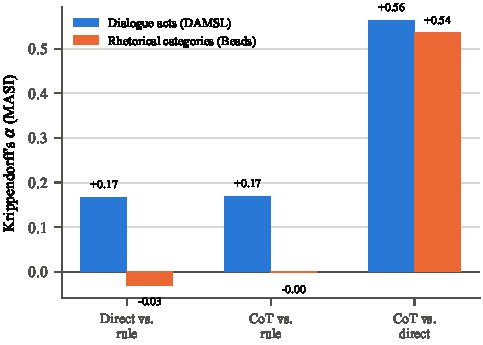
\includegraphics[width=\columnwidth]{figures/fig_cot.pdf}
  \caption{Chain-of-thought prompting does not close the gap with the
  rule-based tagger. Both prompting styles land at the same chance-level
  agreement with the rules; what changes is how much the two LLM conditions
  agree with each other.}
  \label{fig:cot}
\end{figure}

\section{Supplementary Multimodal Models}
\label{app:supplement}

\emph{Weighted sum.} Each measure gets a weight equal to how well it
separates the groups in training debates $T$:
\begin{equation}
w_j \;=\; \frac{1}{|W_T|}\sum_{i \in W_T} z_{ij} \;-\;
          \frac{1}{|L_T|}\sum_{i \in L_T} z_{ij} \,,
\label{eq:weights}
\end{equation}
The weight vector is scaled to unit length. Each sentence is then scored
as $S_i = \sum_{j=1}^{34} w_j z_{ij}$. Weights are learned on $23$ debates
and scored on the twenty-fourth, rotating through all of them.

\begin{table}[h]
\caption{Combining measures, against the two measures that survived on their
own.}
\label{tab:combine}
\centering
\scriptsize
\setlength{\tabcolsep}{2.5pt}
\begin{tabular}{lrrrr}
\toprule
 & \multicolumn{2}{c}{Single measures} & \multicolumn{2}{c}{Composite (34 measures)} \\
\cmidrule(lr){2-3}\cmidrule(lr){4-5}
 & Semitone & Semitone & hold out & hold out \\
 & 20--80 range & SD/mean & debate & speakers \\
\midrule
Mean per-debate effect & $-0.243$ & $\mathbf{-0.370}$ & $+0.390$ & $+0.070$ \\
SD across debates      & $0.289$  & $0.358$  & $0.603$ & $0.519$ \\
Debates in direction   & $21/24$  & $20/24$  & $17/24$ & $11/24$ \\
Sign-test $p$          & $0.0003$ & $0.0015$ & $0.064$ & $0.84$ \\
\bottomrule
\end{tabular}
\end{table}

On held-out debates, the weighted composite reaches $+0.390$ standard
deviations, a $60\%$ improvement on the semitone percentile range alone.
But it is markedly less consistent (SD across debates $0.603$ against
$0.289$). Under speaker holdout it falls to $+0.070$. A single measure
needing no training is more reliable than a weighted combination of $34$.

\emph{Discriminant loadings.} Averaged to the $51$ speaker-by-debate cells,
the discriminant separates winning from non-winning cells at an area under
the curve of $0.907$. Table~\ref{tab:loadings} reports the correlation
between each measure and the discriminant score. Correlations are more
stable than raw weights when measures are correlated.

\begin{table}[h]
\caption{What the discriminant leans on. Positive means higher among winning
candidates.}
\label{tab:loadings}
\centering
\footnotesize
\begin{tabular}{lr}
\toprule
Measure & Loading \\
\midrule
Voice clarity (openSMILE)       & $+0.628$ \\
Semitone pitch SD/mean          & $-0.587$ \\
Voice clarity (Praat)           & $+0.462$ \\
Pitch SD (Hz)                   & $-0.422$ \\
Semitone $20$--$80$ pitch range & $-0.410$ \\
Pitch range (Hz)                & $-0.317$ \\
Articulation rate (syll/s)      & $+0.235$ \\
Mean pitch                      & $+0.189$ \\
Pause duration                  & $+0.186$ \\
Articulation rate (words/s)     & $+0.181$ \\
\bottomrule
\end{tabular}
\end{table}

Every measure in the top ten is acoustic. Nothing syntactic, lexical or
semantic appears until well below. The highest-loading measure is the one
shown in Section~\ref{sec:method:acoustic} to track the speaker's own pitch
at $r = +0.78$ to $+0.90$. Consistent with that, $81.0\%$ of the variance
in the cell scores is explained by which speaker the cell belongs to.

\emph{Principal component analysis.} PCA asks whether the outcome happens to
line up with the largest-variance directions among the $34$ measures without
using the labels at all.

\begin{figure*}[t]
  \centering
  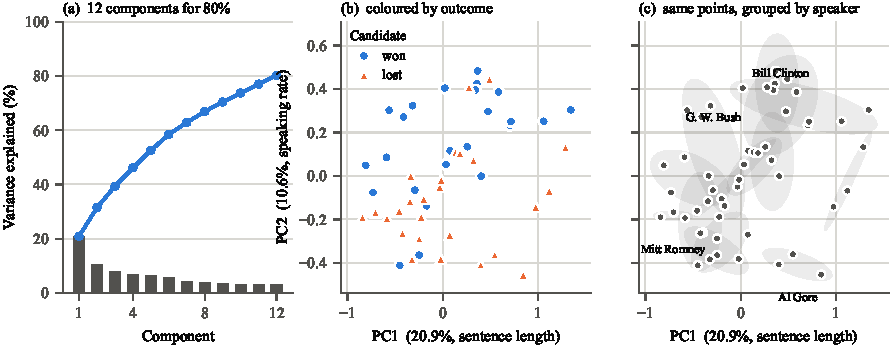
\includegraphics[width=0.99\textwidth]{figures/fig_pca.pdf}
  \caption{Principal component analysis of the $34$ standardised measures.
  (a) Twelve components are needed for $80\%$ of the variance. (b) Each
  point is one candidate in one debate, coloured by outcome. (c) The same
  points, with an ellipse around each speaker's debates. The apparent
  separation by outcome in (b) coincides with the speaker grouping in (c).}
  \label{fig:pca}
\end{figure*}

\begin{table}[h]
\caption{Principal components of the $34$ standardised measures.}
\label{tab:pca}
\centering
\footnotesize
\setlength{\tabcolsep}{3pt}
\begin{tabular}{lrrl}
\toprule
 & \% of & Separation & Dominant measures \\
 & variance & of groups & \\
\midrule
PC1 & $20.9$ & $+0.006$ & Sentence length, grade level \\
PC2 & $10.6$ & $+0.136$ & Articulation rate, speech rate \\
PC3 & $7.9$  & $+0.203$ & Pitch SD, reading ease \\
PC4 & $6.8$  & $+0.070$ & Mean pitch, voice clarity \\
PC5 & $6.4$  & $+0.359$ & Voice clarity (both tools) \\
PC6 & $5.9$  & $+0.044$ & Sentiment \\
\midrule
\multicolumn{4}{l}{$12$ components needed for $80\%$ of variance.} \\
\multicolumn{4}{l}{At cell level, speaker explains $83.6\%$ of PC1 and} \\
\multicolumn{4}{l}{$86.6\%$ of PC2 positions.} \\
\bottomrule
\end{tabular}
\end{table}

PC1 ($20.9\%$ of variance) is a sentence-length dimension separating the
groups at $+0.006$ standard deviations---nothing. PC2 is speaking rate. The
component that best separates the groups is PC5, at $+0.359$, accounting for
only $6.4\%$ of the variance. A hand-built weighted sum, a supervised
discriminant, and an unsupervised decomposition that ignores the labels
entirely all reach the same place: what structure exists in these $34$
measures is mostly about who is speaking.

\emph{LLM ``both'' condition.} Given the transcript and the descriptor
table together, the model calls $24$ of $24$ debates correctly. This
agrees with the transcript-only condition (Section~\ref{sec:llm:accuracy})
on all $24$ debates. Adding numeric descriptors to a transcript the model
can already place in history changes nothing, because the transcript had
already settled the answer.

\section{LLM Methods and Reproducibility}
\label{app:llmrepro}

This appendix specifies every language-model call in the paper: the original
discourse tagging and its chain-of-thought variant (Appendix~\ref{app:tagging}),
and the cross-modal winner prediction with its contamination probe
(Sections~\ref{sec:method:llmprotocol}, \ref{sec:method:llm}). The goal is
that another researcher could reissue every call from this description
alone.

\emph{Model.} All components use the same model, \texttt{claude-opus-4-8},
accessed through Anthropic's Messages API. Anthropic does not publish a
parameter count for this model, so none is reported here. Reporting one
would imply a precision we do not have. Every call uses structured
(\texttt{json\_schema}) output: the model's response is constrained at
generation time to match a schema we specify, rather than parsed after the
fact from free text. All calls were issued on $2026$-$08$-$06$.

\emph{Sampling.} This model deprecates the \texttt{temperature} parameter.
The API rejects a request that sets it. Repeated calls therefore draw on
whatever sampling variability the API applies by default, not on a
caller-chosen temperature. Where the paper reports a repeat count, that is
the only lever available for measuring stability.

\emph{Discourse tagging.} System prompt, codebook and full JSON schema are
reproduced verbatim in \texttt{Sahana Project/tagging\_prompt.md} (direct)
and \texttt{Sahana Project/cot\_tagging\_prompt.md} (chain-of-thought). Both
send $10$ sentences per request, batched for throughput, with the system
prompt and codebook cached (\texttt{cache\_control: ephemeral}) across
requests. The only schema difference is one field, \texttt{reasoning}, which
the chain-of-thought variant requires before \texttt{damsl} and
\texttt{beads}. Structured output fills schema fields in the order they
are declared. This forces the free-text reasoning to be generated before
the codes rather than after them.

\emph{Cross-modal winner prediction.} System prompt, both JSON schemas
(descriptor-citing and theme-citing), the contamination-probe prompt and
schema, and the closed evidence vocabularies are reproduced verbatim in
\texttt{Sahana Project/crossmodal\_prompt.md}. One call is issued per debate,
per condition, per repeat. Each repeat uses a freshly randomised
Candidate-A/B/C letter assignment, shared across conditions within that
repeat so predictions are comparable trial-for-trial. The contamination
probe issues one further call per debate per input type, with no repeats.
It is a single-shot identification question rather than a graded
judgement. Every
call uses a fresh, empty context, so agreement or disagreement between
conditions reflects the input alone.

\emph{Anonymisation.} Candidate names, party affiliation and the debate
date are removed from every input. Moderator turns are dropped entirely,
leaving only candidate sentences in original chronological order. This is
a partial defence at best. A transcript's content---quoted lines, named
policies, the other candidate's real name spoken aloud mid-turn---was not
scrubbed. Removing it would have taken out the communicative content the
transcript condition exists to test. The contamination probe measures what
leaks through this partial anonymisation rather than assuming it is
complete. All $24$ of $24$ transcripts were identified regardless of the
redaction.

\emph{Grounding check.} A cited measure counts as consistent with a
debate's real data when the candidate it names as favoured actually has
the higher within-debate standardised value for that measure. A margin of
less than $0.15$ standard deviations between the two candidates is scored
as ``similar'' and excluded rather than forced to a side. This is an
automatic, closed-vocabulary check, not a human judgement of whether the
reasoning sounds plausible.

\section{Exploratory Same-Candidate Analysis}
\label{app:samecand}

\begin{table}[h]
\caption{Where the same speaker lands when they won and when they lost. The
discriminant was fitted \emph{without} that speaker, then their debates
projected in. Scores are relative to the opponent on the night.}
\label{tab:within}
\centering
\footnotesize
\begin{tabular}{llcr}
\toprule
Speaker & Debate & Outcome & Score \\
\midrule
\multirow{5}{*}{G.\,H.\,W.\ Bush}
 & 1988, first  & won  & $-0.021$ \\
 & 1988, second & won  & $-0.066$ \\
 & 1992, first  & lost & $-0.224$ \\
 & 1992, second & lost & $-0.203$ \\
 & 1992, third  & lost & $-0.223$ \\
\cmidrule(lr){2-4}
 & \multicolumn{2}{l}{gap (won $-$ lost)} & $+0.173$ \\
 & \multicolumn{2}{l}{winning above losing} & $6/6$ \\
\midrule
\multirow{5}{*}{Donald Trump}
 & 2016, first  & won  & $+0.010$ \\
 & 2016, second & won  & $-0.018$ \\
 & 2016, third  & won  & $-0.025$ \\
 & 2020, first  & lost & $-0.034$ \\
 & 2020, second & lost & $+0.002$ \\
\cmidrule(lr){2-4}
 & \multicolumn{2}{l}{gap (won $-$ lost)} & $+0.005$ \\
 & \multicolumn{2}{l}{winning above losing} & $4/6$ \\
\bottomrule
\end{tabular}
\end{table}

\section{2024 Exclusion and Known Corpus Issues}
\label{app:known}

Two 2024 debates exist in the corpus but are held out, because we could
not verify who was speaking. Their official transcripts are paraphrased
news summaries, sharing only $5.2\%$ and $5.5\%$ of their words with the
audio. As a result, the recognised text was used as the transcript, and
speakers were assigned by diarization \cite{bredin2023pyannote}. That
diarization was never checked against hand-labelled data. We have no
error rate for it.

Four things prompted the exclusion. In the June 2024 debate one candidate is
credited with $786$ sentences and the other with $256$---three to one, in a
format with timed turns and muted microphones. In the September debate about
$285$ sentences sit in twelve or more leftover speaker clusters. Across the
pair, $1{,}162$ sentences are labelled \emph{audience}, in two debates with no
audience. Finally, candidates account for $43.9\%$ of sentences in these
two, against $76$ to $86\%$ everywhere else.

The confirmation is what happens on removal: across the remaining $24$
debates, unattributed sentences drop to zero and audience sentences to $287$.
All of the unattributed material and $80.2\%$ of the audience material came
from those two debates. Including the pair changes several results. Noun
rate flips sign, from $-0.012$ to $+0.043$. Sentiment roughly halves. The
embedding axis rotates (cosine similarity $0.895$ to the one reported
here). Finally, $19$ of the $50$ most extreme sentences at one end come
from this $9.5\%$ of the data. These transcripts also contain no
truncation marks and no filled pauses at all. As a result, interruption
and self-correction are missing by construction.

\subsection*{Availability}
The corpus is deposited with a permanent identifier. Released material covers
the annotation layers, the per-sentence features and the checking scripts.
Alignment scripts point at audio sourced elsewhere, which cannot be
redistributed. A data statement, a column dictionary and the annotation
codebook accompany the deposit.
\label{app:resource}

\subsection*{Known problems}
\begin{itemize}\itemsep1pt
  \item $25$ candidate sentences of eight words or more are exact duplicates
        within a debate, $17$ of them in the first 1988 debate. One pair has
        the same text attributed to two different candidates, so speaker
        attribution is not verified anywhere in the corpus.
  \item $8$ candidate rows share an identical time span---one group of nine
        sentences assigned a zero-length window.
  \item $238$ candidate rows have no duration, almost all in one debate.
        That debate is also where every extraction error occurs.
  \item Acoustic extraction fails on $4.5\%$ of candidate rows: $3.2\%$ too
        short, $0.9\%$ errors, split $2.8\%$ against $16.5\%$ across the two
        alignment treatments.
  \item No two candidate sentences overlap in time, so interruptions are not
        represented.
  \item Two rule-based categories duplicate the sentence-type column, and
        $13$ codes never fire, both discussed in Appendix~\ref{app:tagging}.
\end{itemize}

\end{appendices}

\bibliography{refs}

\end{document}
